\chapter{Fit Supplementaries}
\label{chap:apdx_fitsupp}
%In this appendix we list some additional visualizations related to the fit model that we established in Chap.~\ref{chap:fit}:
%In Fig.~\ref{fig:fit_hLbM_MC_Lb} and Fig.~\ref{fig:fit_hLbM_MC_Xib} we show the fit projections of a double Gaussian shape to the invariant mass distributions of \Dz and \Lz candidates of MC generated \decay{\Lb}{\Dz\Lz} and \decay{\Xibz}{\Dz\Lz} decays of both track types.
%Whereas in Fig.~\ref{fig:fit_hLbM_data_fit1} we showed the accumulated fit projection to both track types for recorded data, we show in Fig.~\ref{fig:fit_hLbM_data_fit1_LLDD} the track type dependent fit projection, as well as the accumulated projection (and log-likelihood value) if one signal component is deactivated as used for estimating the signal significance in Fig.~\ref{fig:fit_hLbM_data_fit23}.
%In Fig.~\ref{fig:fit_hLbM_data_fit1_LLDD_tis} (Fig.~\ref{fig:fit_hLbM_data_LLDD_otos}) we show the fit results (data distribution) when recorded data are required to have a positive (negative) \gls{lzero} \gls{tis} trigger decision.
%In Fig.~\ref{fig:fit_hLbM_data_fit4} we show the fit projection for recorded data in configuration 4. In comparison with configuration 3 (\cf{}~Fig.~\ref{fig:fit_hLbM_data_fit3}), here the \Dstarz ratio is allow to vary among different track types.
%
%Finally, we show the \glspl{pdf} used for generating the pseudo-experiments in Fig.~\ref{fig:fit_toy_pdf_cdf} as well as an example of the fit projection to a pseudo-experiment with both signal modes enabled (as used for estimating the bias and the validation of the error estimates) and an example of fits used for verifying the signal yield significance estimation in Fig.~\ref{fig:fit_hLbM_toy_full_fit3} and Fig.~\ref{fig:fit_hLbM_toy_noLb}, respectively.

\begin{table}[htbp]
    \centering
    \caption{Fit results of configuration 1, using the narrow mass range $5.5 \le m(\Dz\Lz) \le 6\,\gevcc$. The value of $f_{\Dstar}$ (marked with $\dagger$) is fixed to zero. All other values are floating parameters during the likelihood maximization.}
    \label{tab:fit_fitres1}
    \begin{tabular}{llll}
        \toprule
        & \multicolumn{2}{c}{{Value}} & \\
        Parameter & \multicolumn{1}{c}{\gls{LL}} & \multicolumn{1}{c}{\gls{DD}} & Unit \\
        \midrule
        $\mu(\Lb)$ & \multicolumn{2}{c}{\num[separate-uncertainty=false]{5.62114 \pm 0.00021}} & \gevcc \\
        $\mu(\Xib)$ & \multicolumn{2}{c}{\num[separate-uncertainty=false]{5.79495 \pm 0.00021}} & \gevcc \\
        $\Delta\mu(\Lb)$ & \multicolumn{2}{c}{\num[separate-uncertainty=false]{0.00162 \pm 0.00032}} & \gevcc \\
        $\Delta\mu(\Xib)$ & \multicolumn{2}{c}{\num[separate-uncertainty=false]{0.00131 \pm 0.00031}} & \gevcc \\
        $\sigma_1(\Lb)$ & \num[separate-uncertainty=false]{0.01435 \pm 0.00028} & \num[separate-uncertainty=false]{0.0151 \pm 0.0007} & \gevcc \\
        $\sigma_1(\Xib)$ & \num[separate-uncertainty=false]{0.01442 \pm 0.00035} & \num[separate-uncertainty=false]{0.0158 \pm 0.0005} & \gevcc \\
        $\sigma_2(\Lb)$ & \num[separate-uncertainty=false]{0.0346 \pm 0.0027} & \num[separate-uncertainty=false]{0.0248 \pm 0.0016} & \gevcc \\
        $\sigma_2(\Xib)$ & \num[separate-uncertainty=false]{0.0283 \pm 0.0017} & \num[separate-uncertainty=false]{0.0280 \pm 0.0018} & \gevcc \\
        $f_\mathcal{G}(\Lb)$ & \num[separate-uncertainty=false]{0.903 \pm 0.021} & \num[separate-uncertainty=false]{0.72 \pm 0.09} & \\
        $f_\mathcal{G}(\Xib)$ & \num[separate-uncertainty=false]{0.838 \pm 0.035} & \num[separate-uncertainty=false]{0.81 \pm 0.05} & \\
        $f_s$ & \multicolumn{2}{c}{\num[separate-uncertainty=false]{0.83 \pm 0.10}} & \\
        $k$ & \num[separate-uncertainty=false]{5.2 \pm 1.6} & \num[separate-uncertainty=false]{2.1 \pm 1.0} & $1 / (\gevcc)$ \\
        $f_{\Dstar}$ & \multicolumn{2}{c}{$0^\dagger$} & \\
        $f_1$ & \num[separate-uncertainty=false]{0.62 \pm 0.10} & \num[separate-uncertainty=false]{0.77 \pm 0.08} & \\
        $f_2$ & \multicolumn{2}{c}{\num[separate-uncertainty=false]{1.0 \pm 0.7}} & \\
        \bottomrule
    \end{tabular}
\end{table}


\begin{figure}[htbp]
    \centering
    \begin{subfigure}[b]{.49\textwidth}
        \centering
        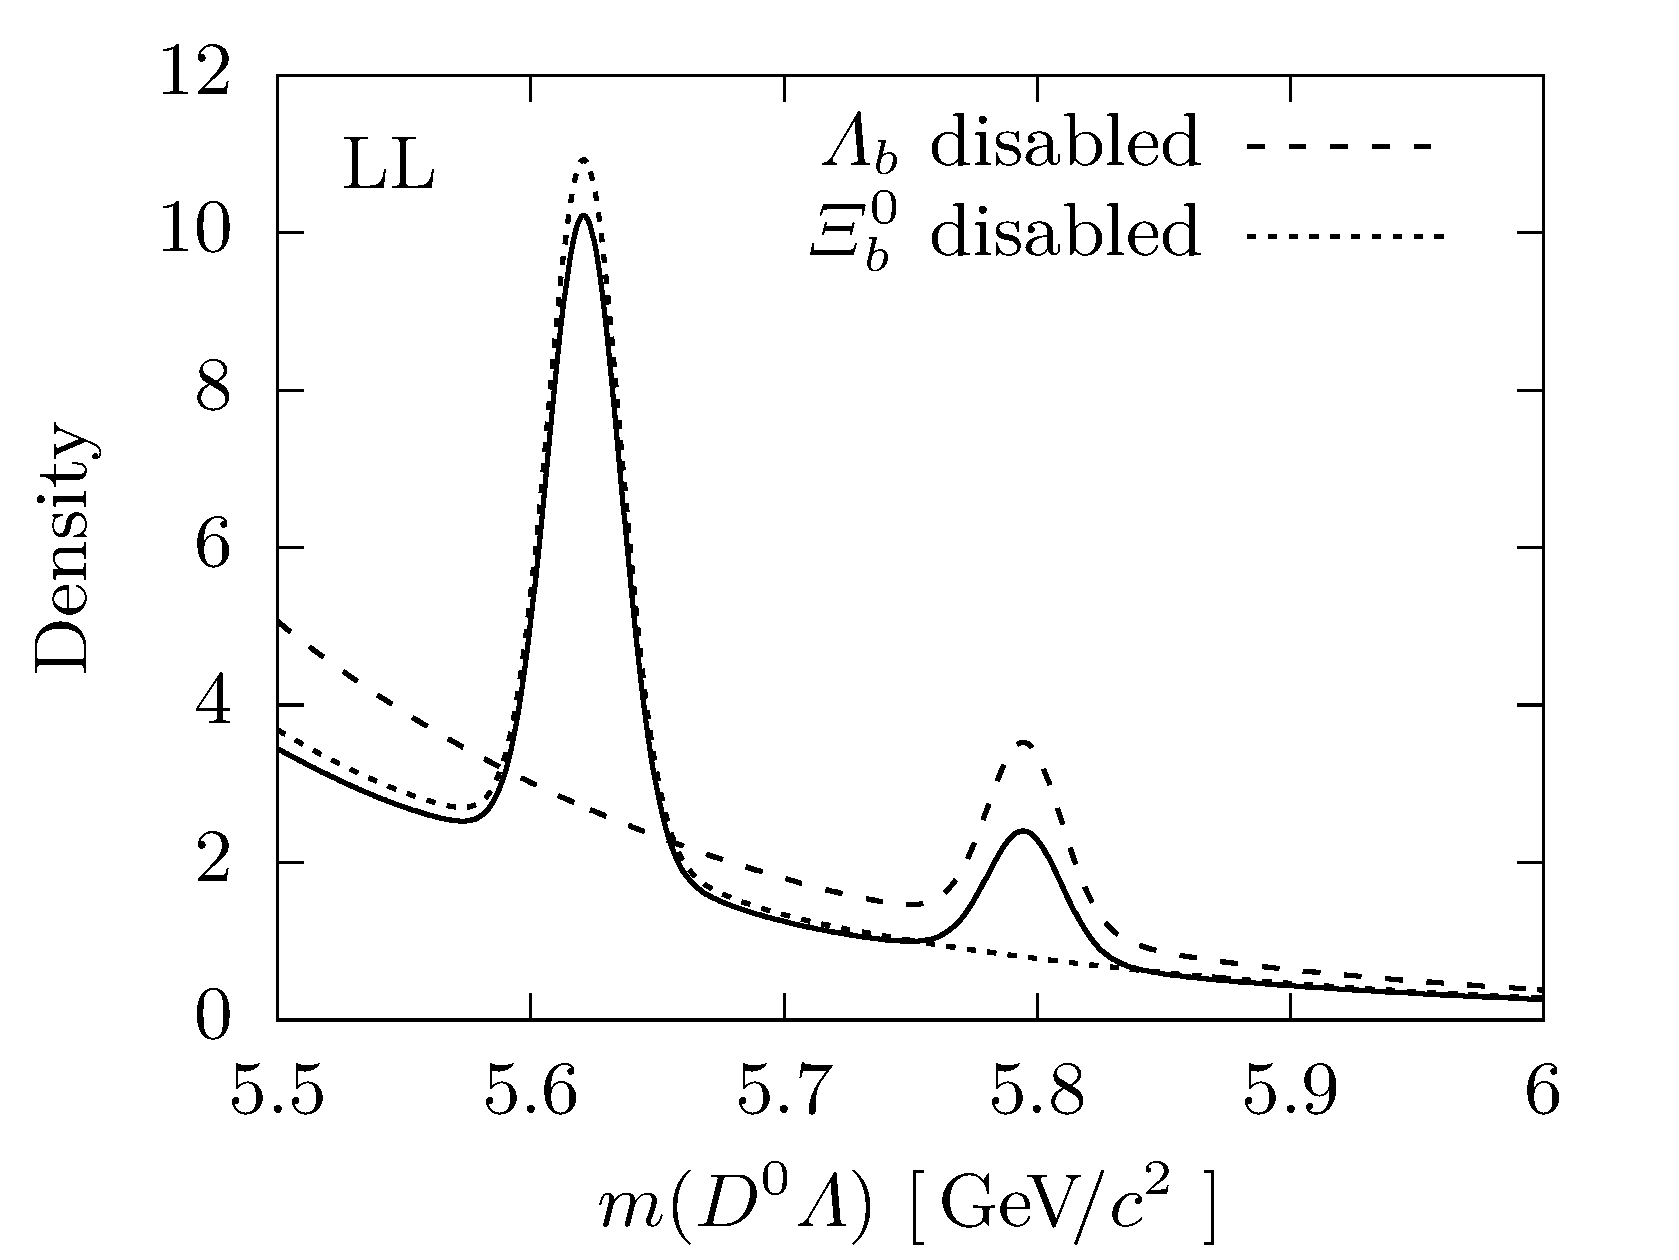
\includegraphics[scale=1.]{fit/pdf_LL.png}
    \end{subfigure}
    \begin{subfigure}[b]{.49\textwidth}
        \centering
        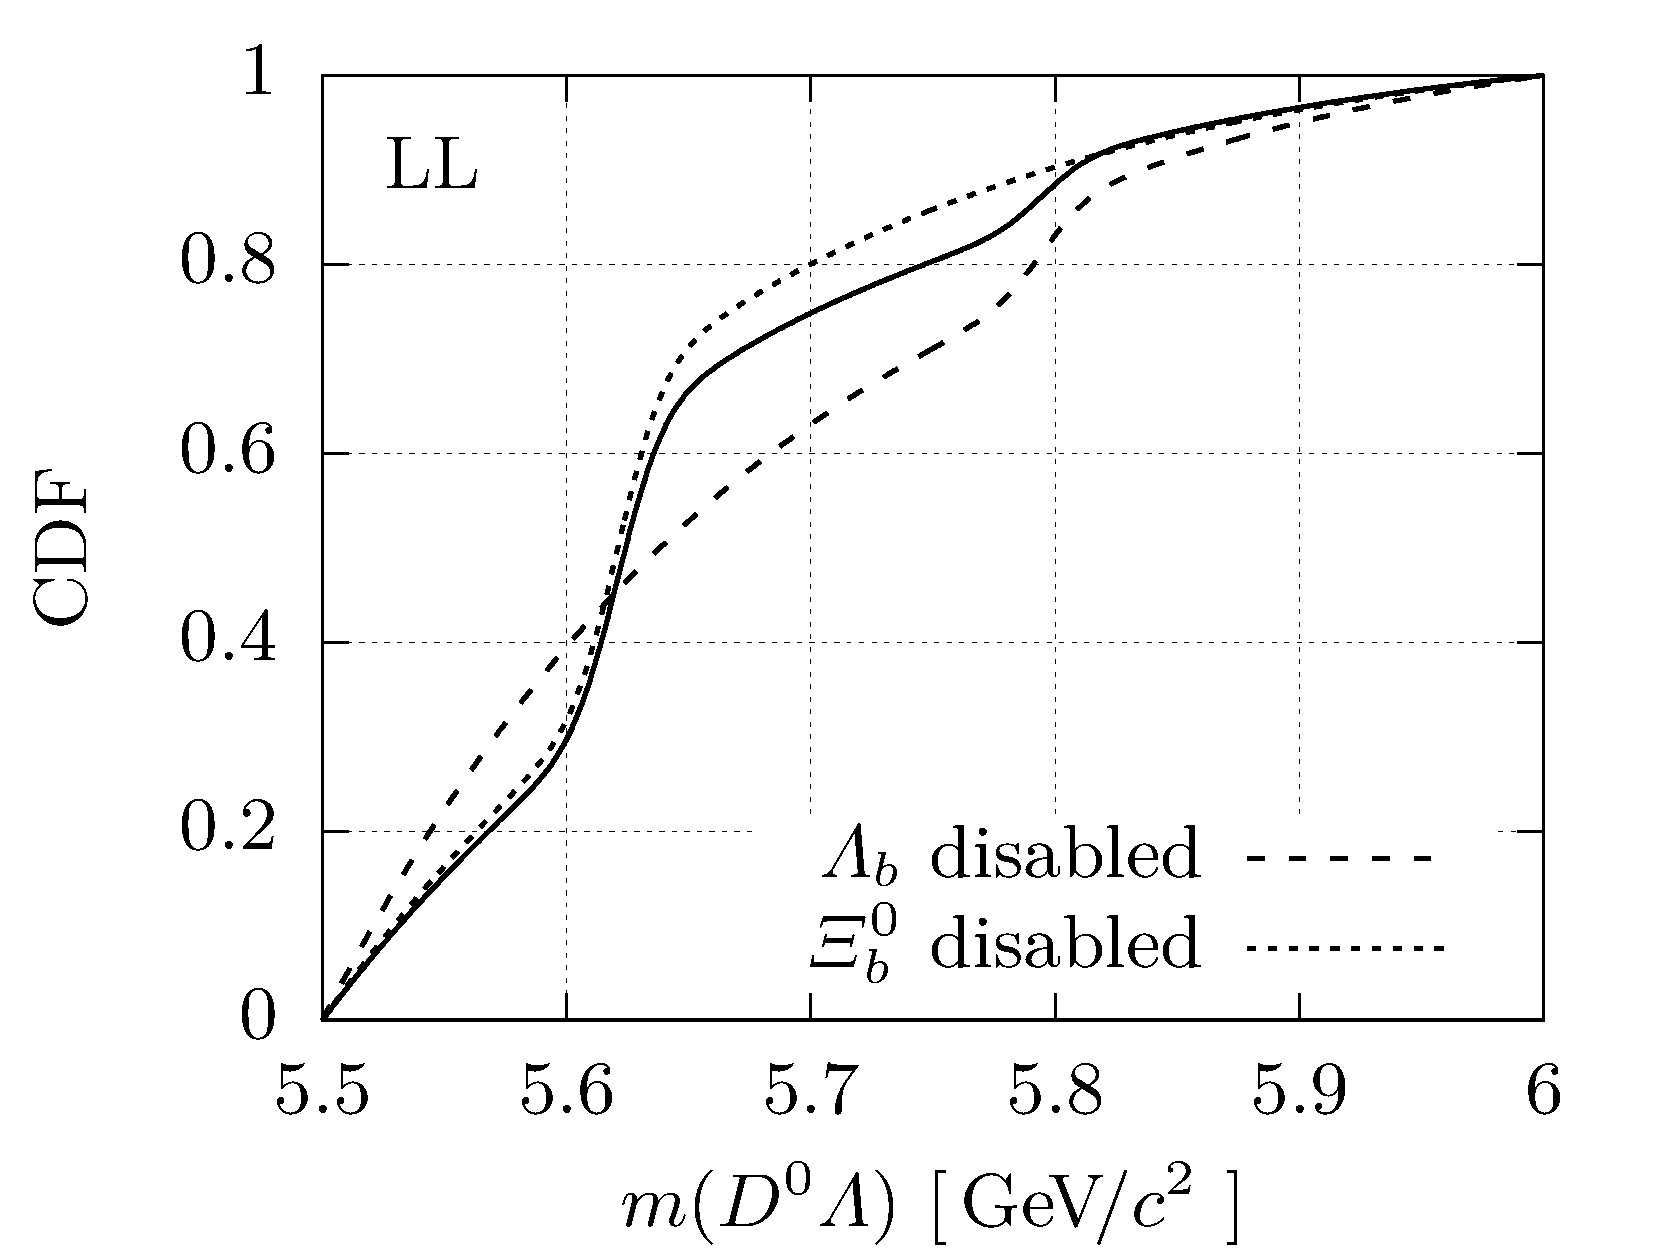
\includegraphics[scale=1.]{fit/cdf_LL.png}
    \end{subfigure}
    \caption{\Glspl{pdf} (left) and their cumulative distributions (right) as fitted in the projection of \gls{LL} tracks in configuration 1 (solid line), as well as the shapes with disabled \decay{\Lb}{\Dz\Lz} or \decay{\Xibz}{\Dz\Lz} component (dashed lines). The cumulative distributions (CDF) are used for generating the pseudo-experiments.}
    \label{fig:fit_toy_pdf_cdf}
\end{figure}

\begin{figure}[htbp]
    \centering
    \begin{subfigure}[b]{.49\textwidth}
        \centering
        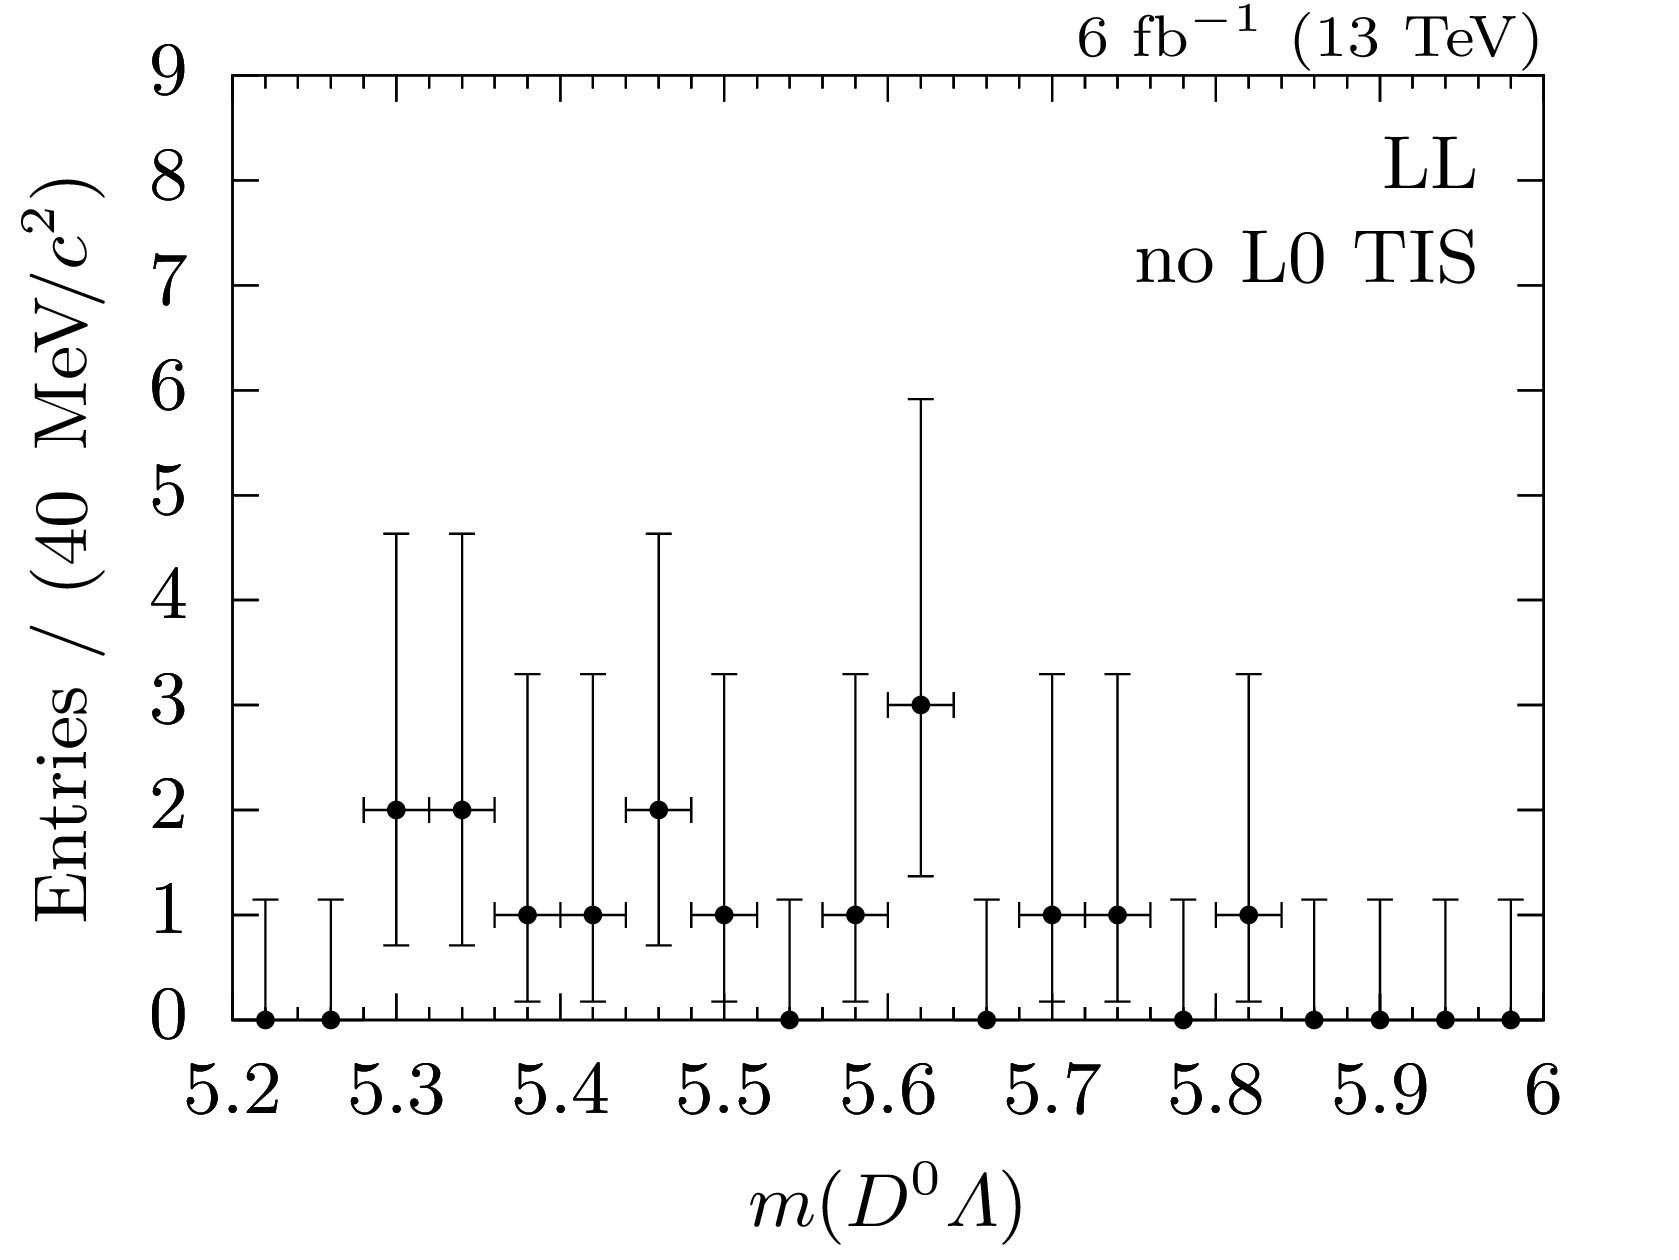
\includegraphics[scale=1.]{fit/hLbM_data_LL_otos.png}
    \end{subfigure}
    \begin{subfigure}[b]{.49\textwidth}
        \centering
        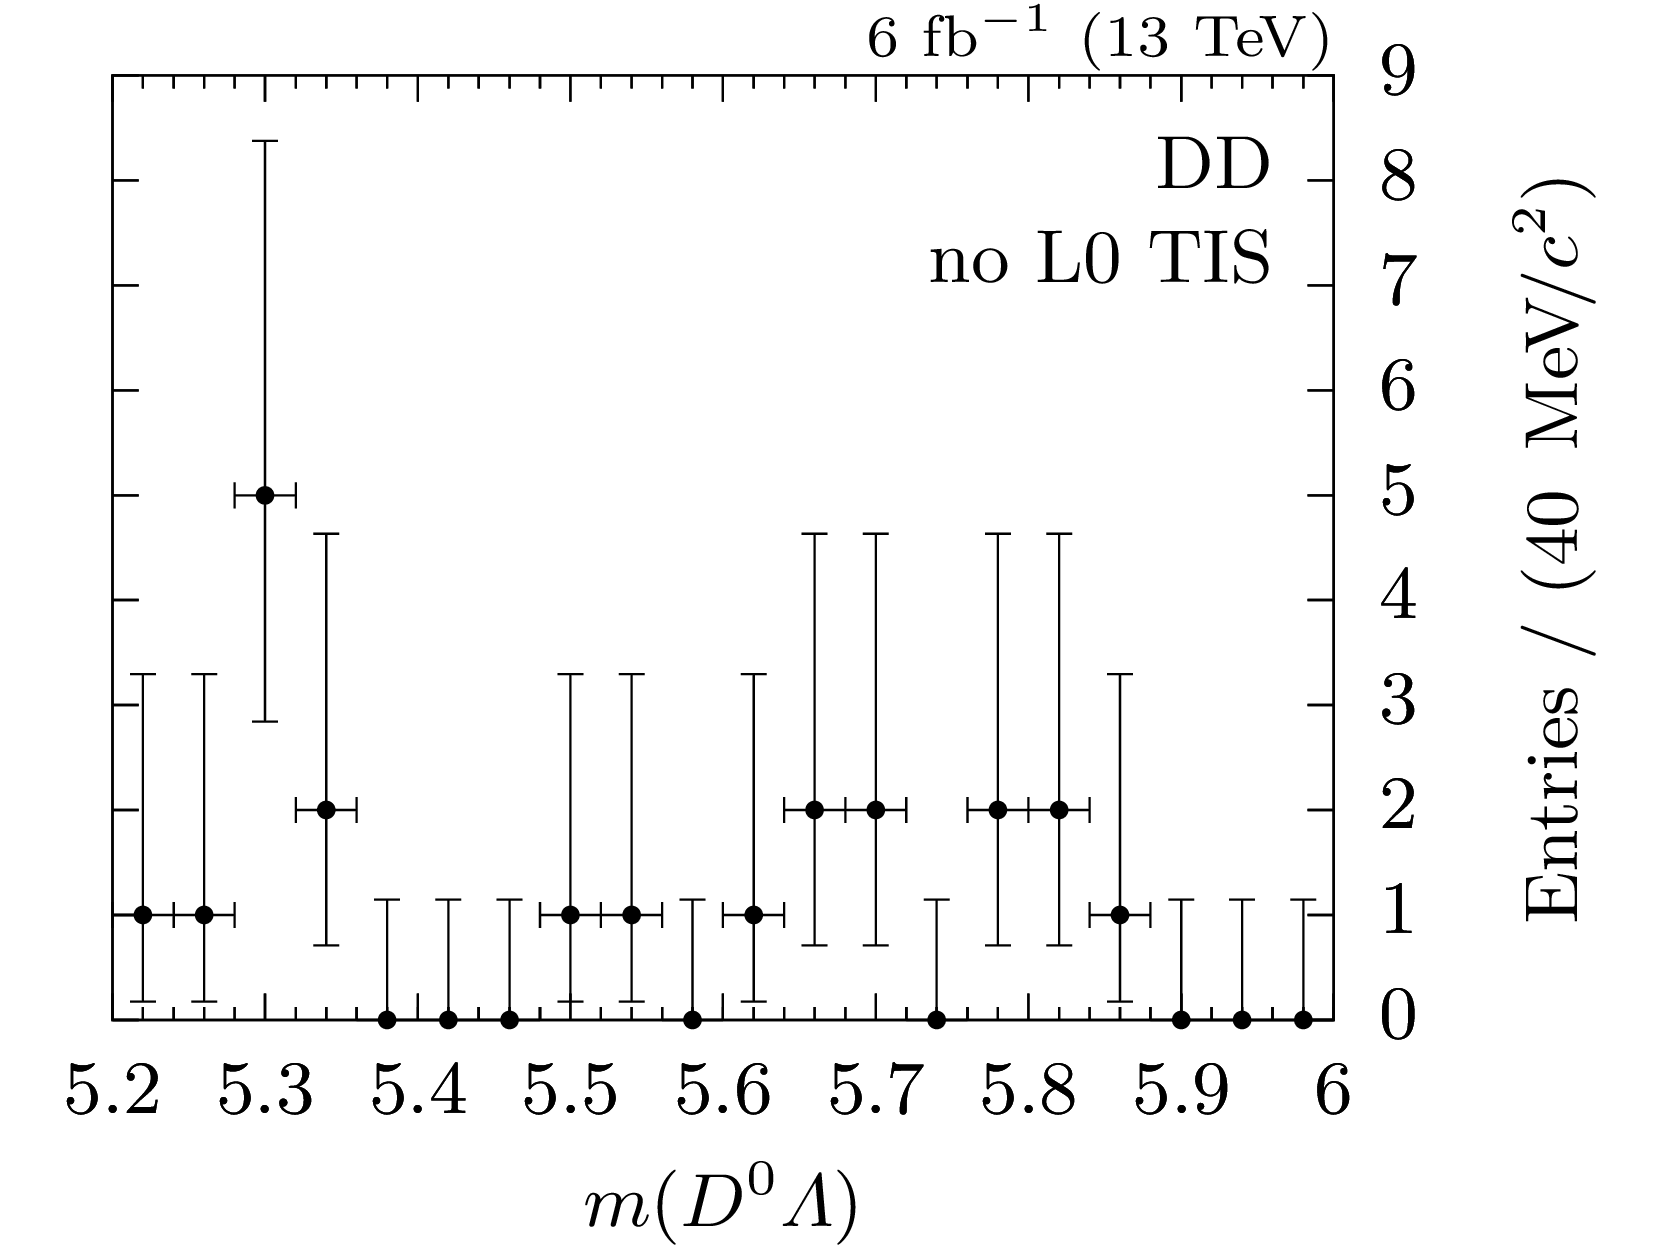
\includegraphics[scale=1.]{fit/hLbM_data_DD_otos.png}
    \end{subfigure}
    \caption{Combined invariant mass of \Dz and \Lz candidates of track type \gls{LL} (left) and \gls{DD} (right) from recorded data with a negative \gls{lzero} \gls{tis} trigger decision.}
    \label{fig:fit_hLbM_data_LLDD_otos}
\end{figure}


\begin{figure}[htbp]
    \centering
    \begin{subfigure}[b]{\textwidth}
        \centering
        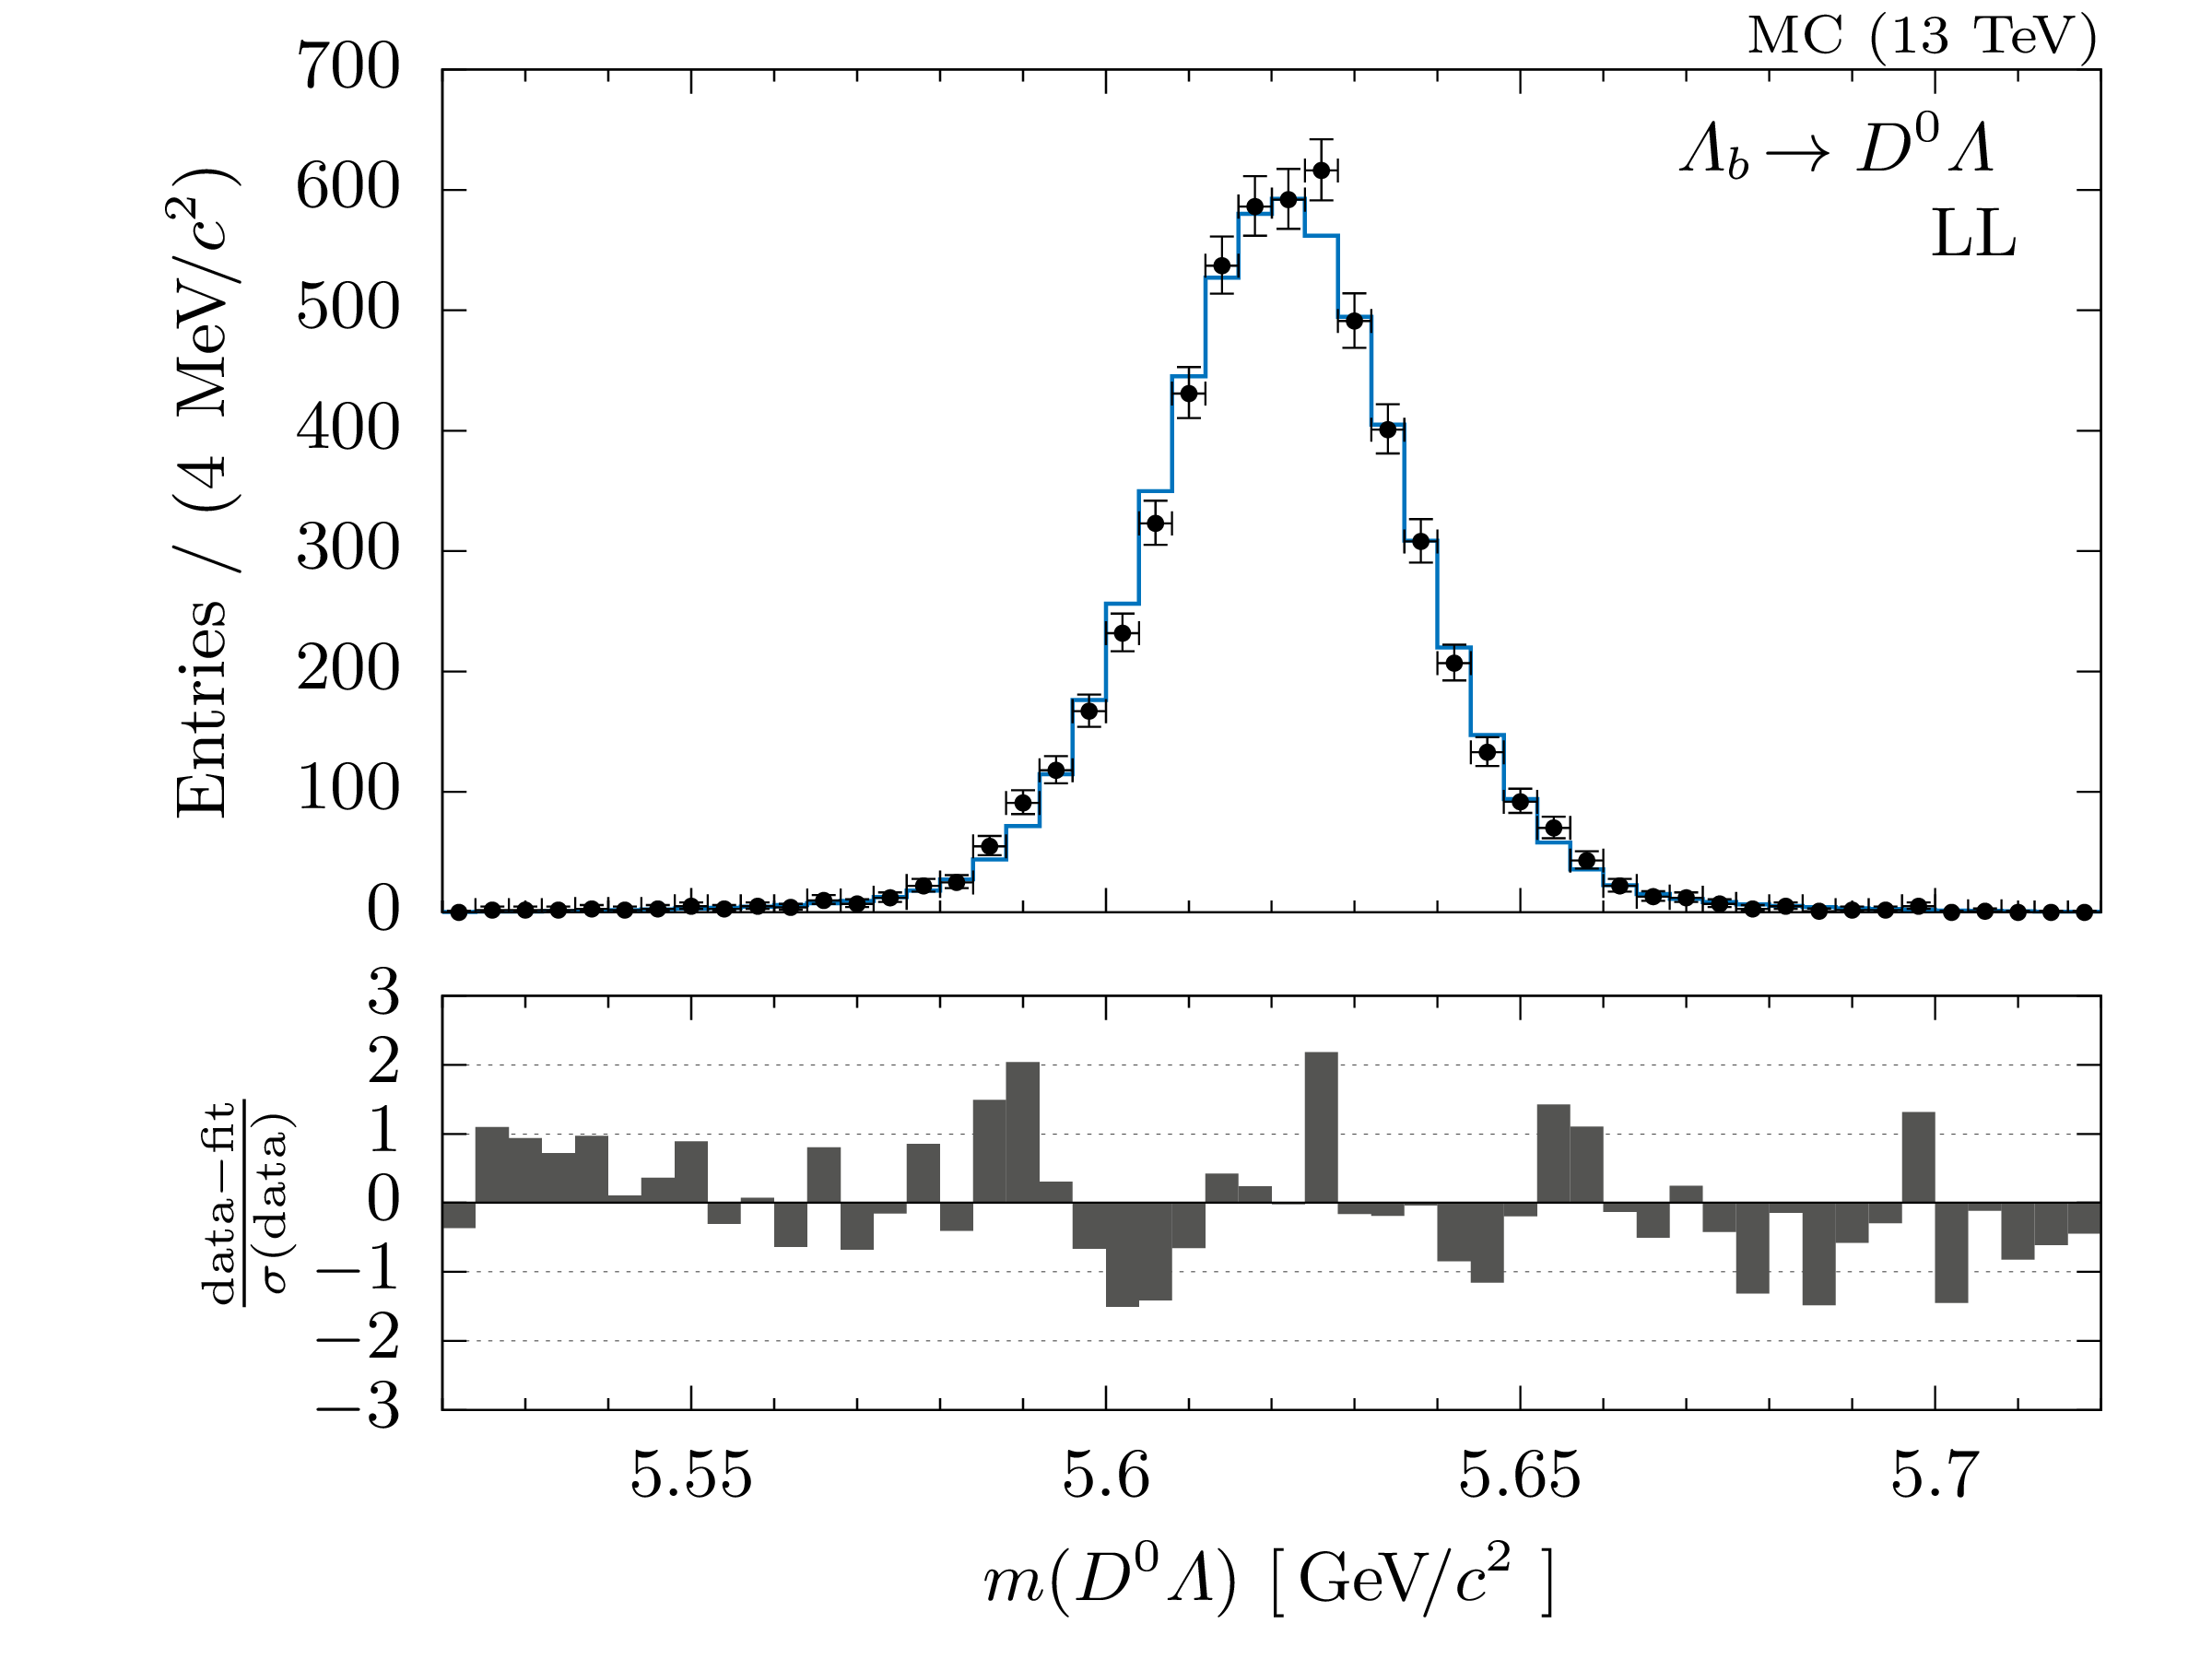
\includegraphics[scale=1.]{fit/hLbM_LL_MC_Lb.png}
    \end{subfigure}
    \par\bigskip 
    \begin{subfigure}[b]{\textwidth}
        \centering
        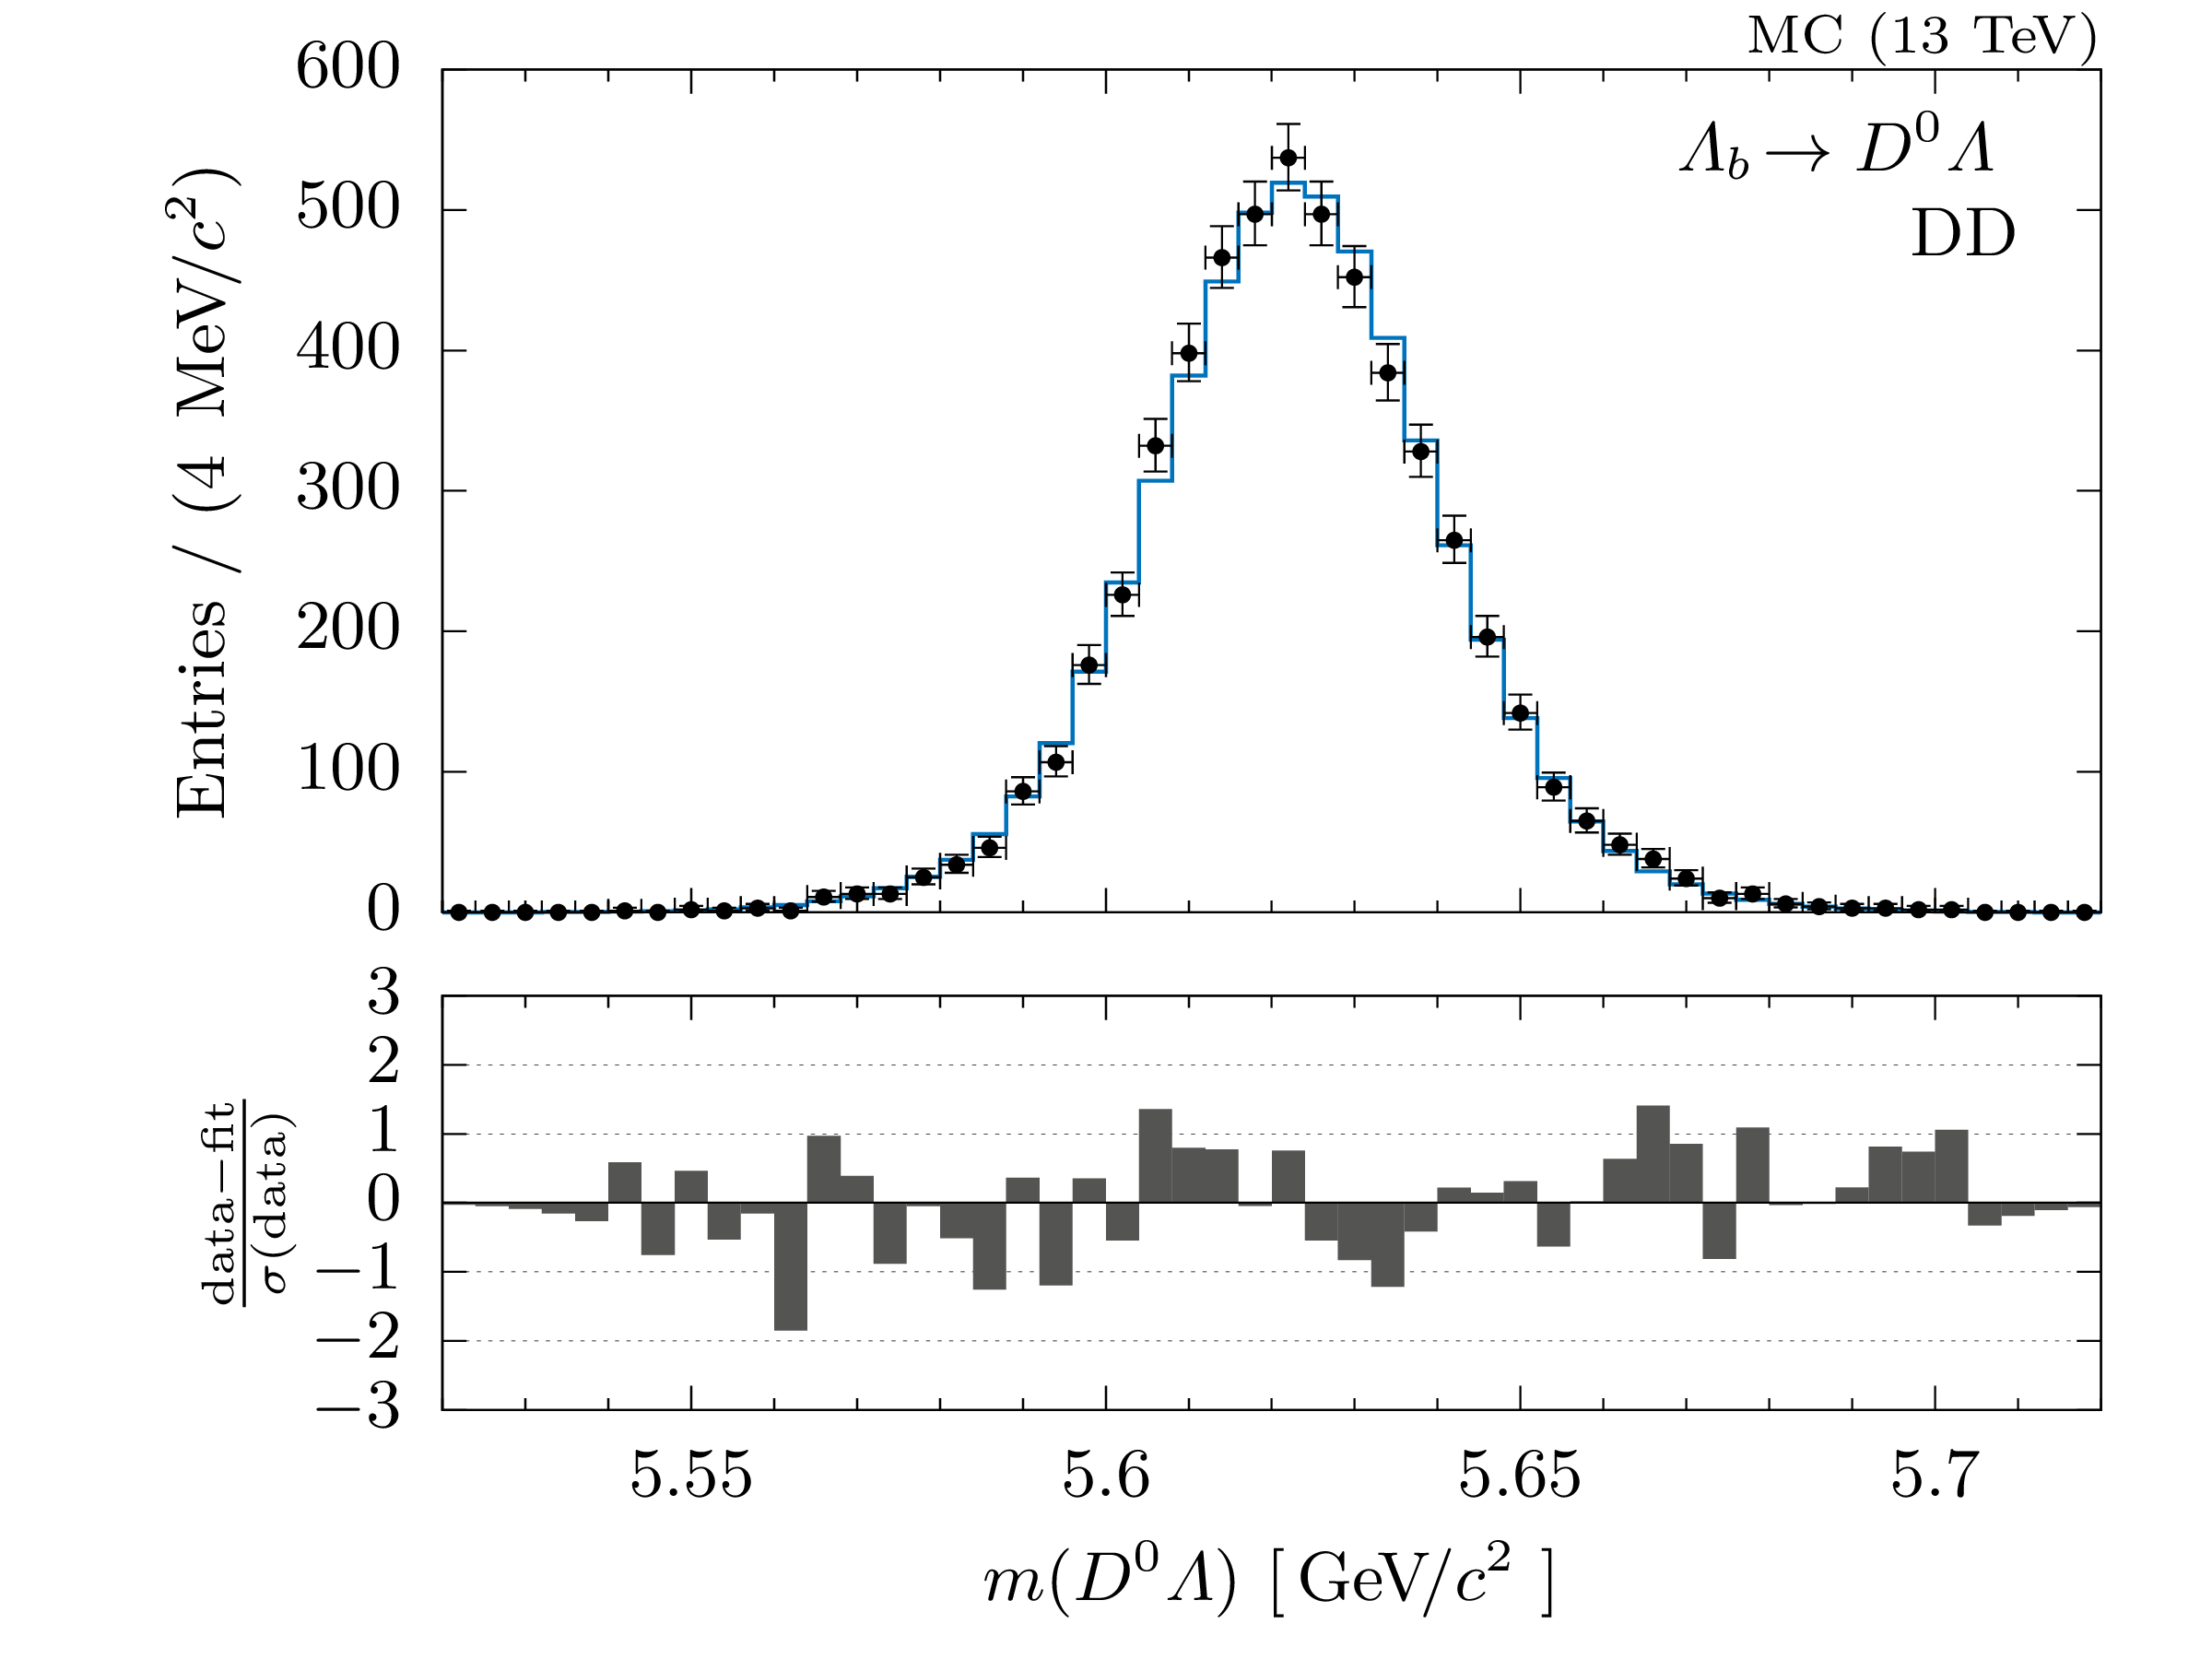
\includegraphics[scale=1.]{fit/hLbM_DD_MC_Lb.png}
    \end{subfigure}
    \caption{Combined invariant mass of \Dz and \Lz candidates of track type \gls{LL} (top) and \gls{DD} (bottom) from \gls{mc} simulated \decay{\Lb}{\Dz\Lz} decays, as well as the corresponding projections of the simultaneous fit in configuration 1.}
    \label{fig:fit_hLbM_MC_Lb}
\end{figure}

\begin{figure}[htbp]
    \centering
    \begin{subfigure}[b]{\textwidth}
        \centering
        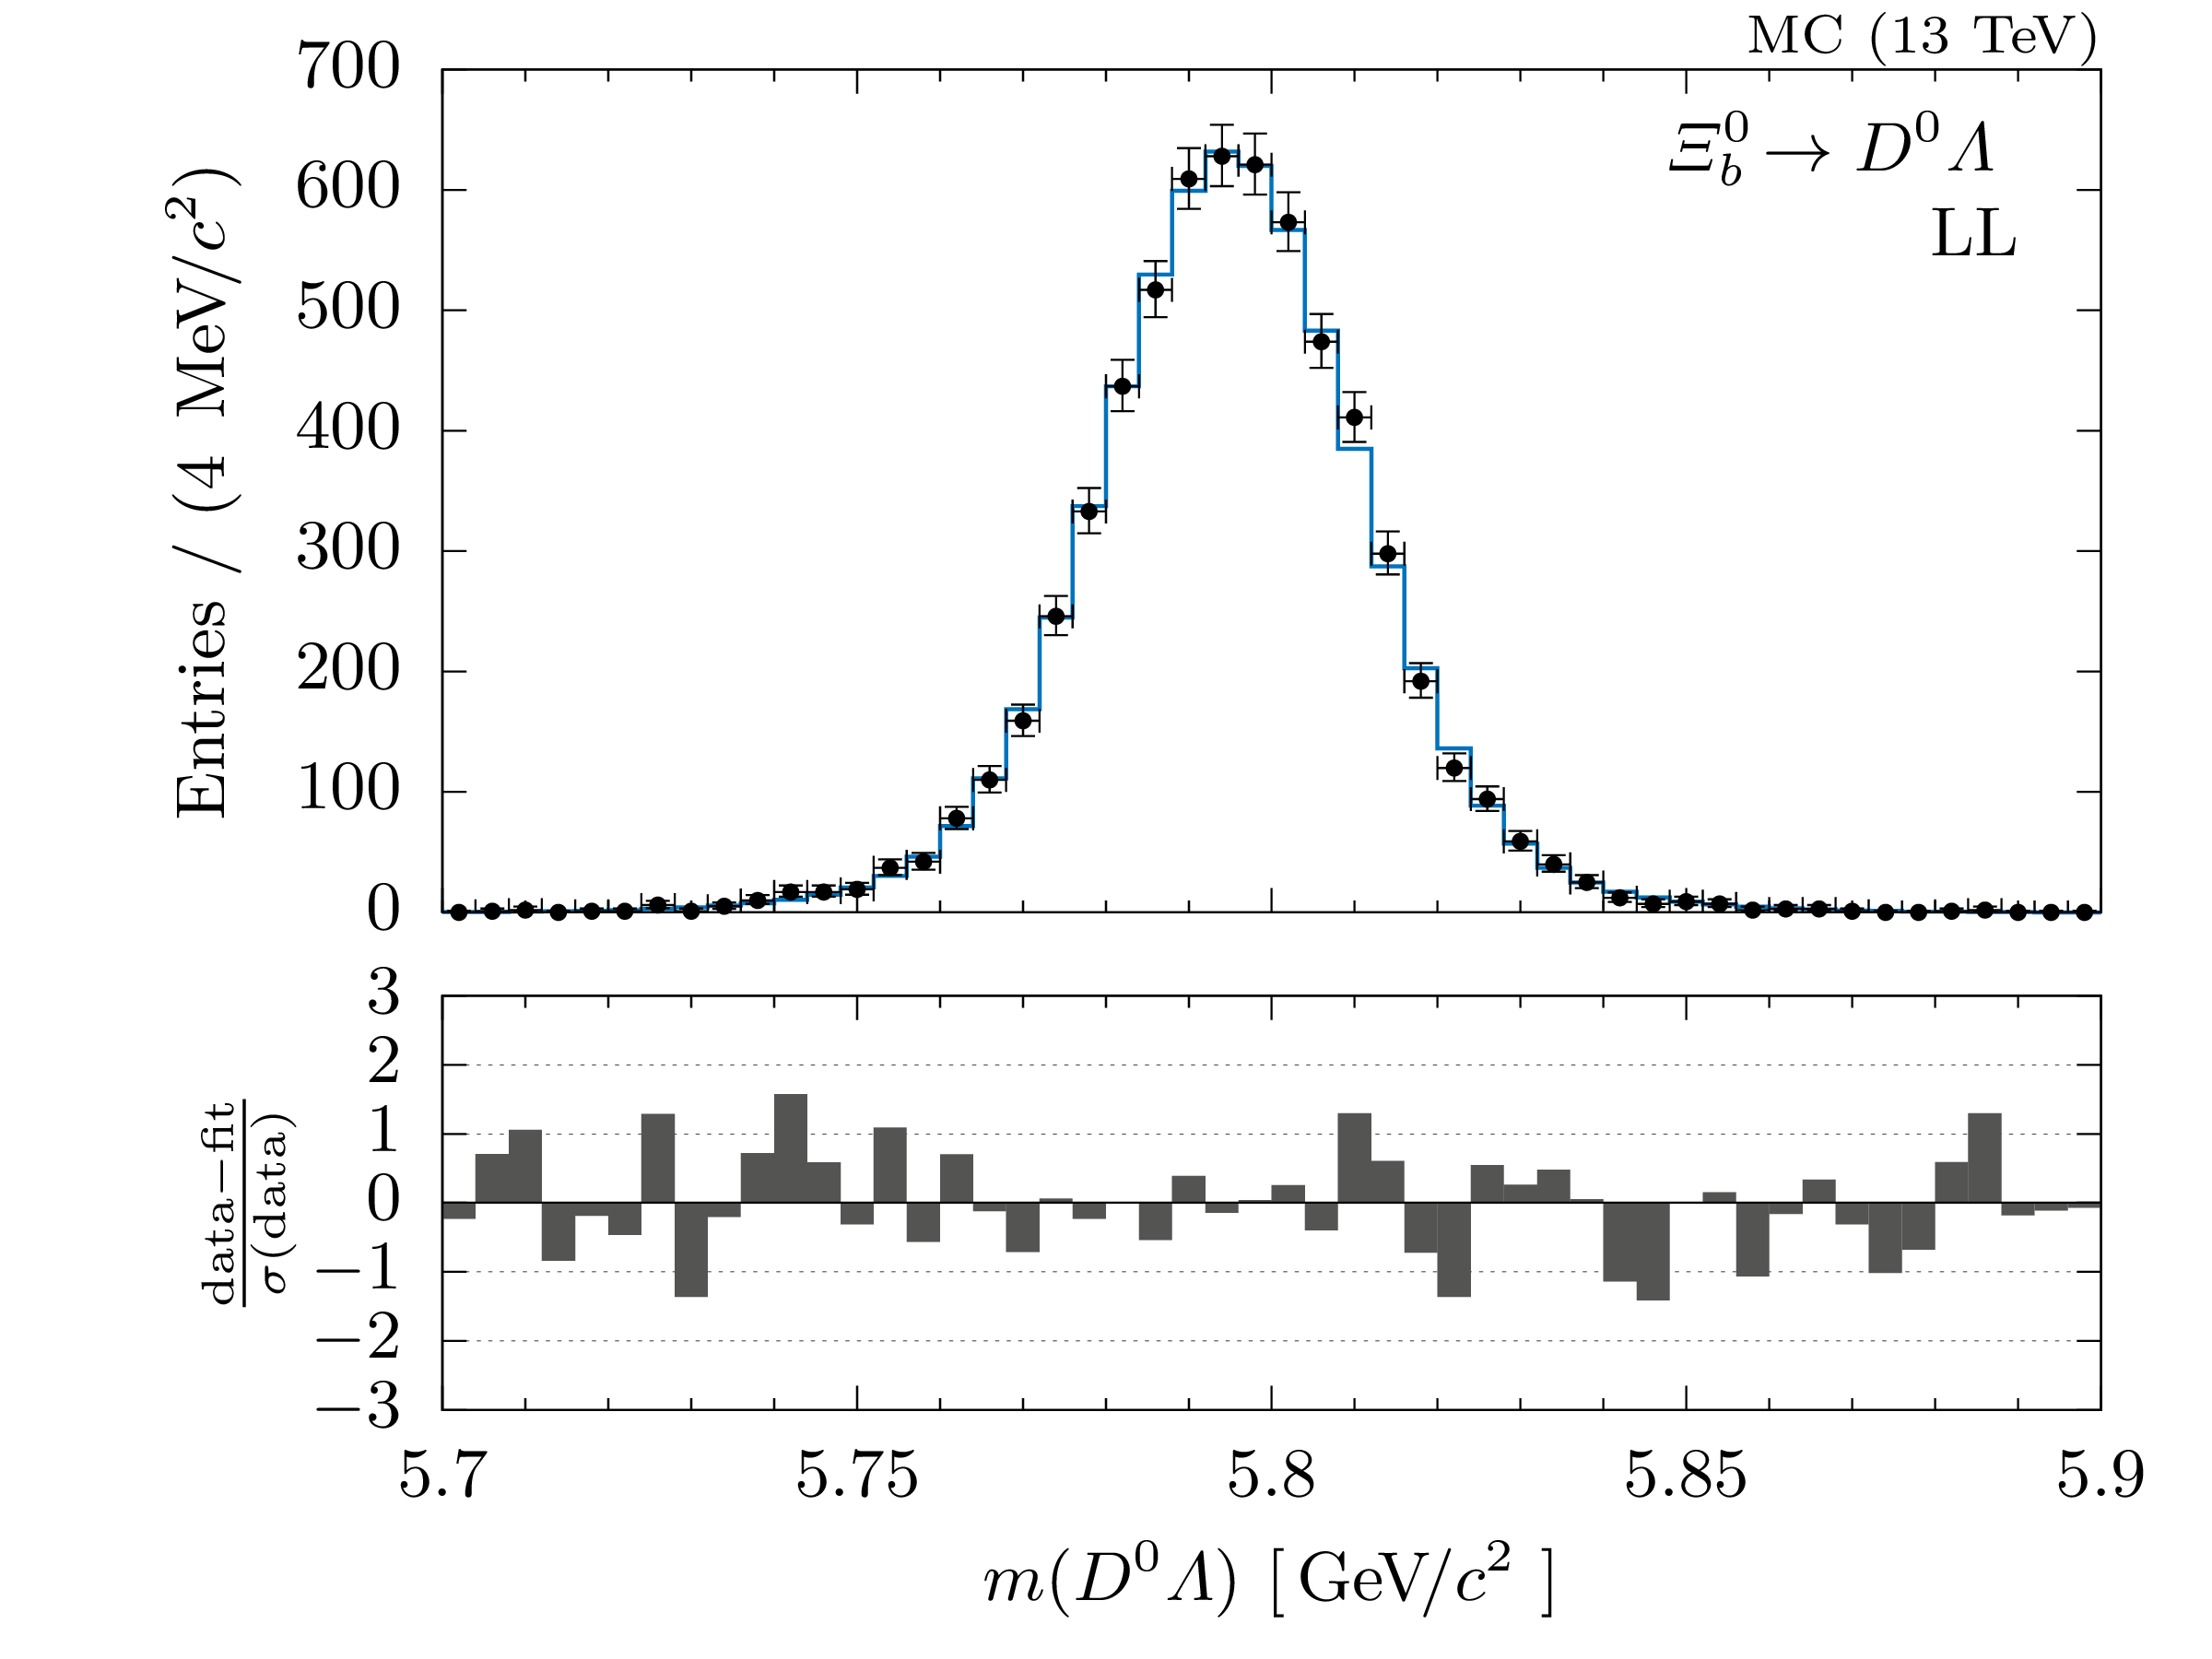
\includegraphics[scale=1.]{fit/hLbM_LL_MC_Xib.png}
    \end{subfigure}
    \par\bigskip 
    \begin{subfigure}[b]{\textwidth}
        \centering
        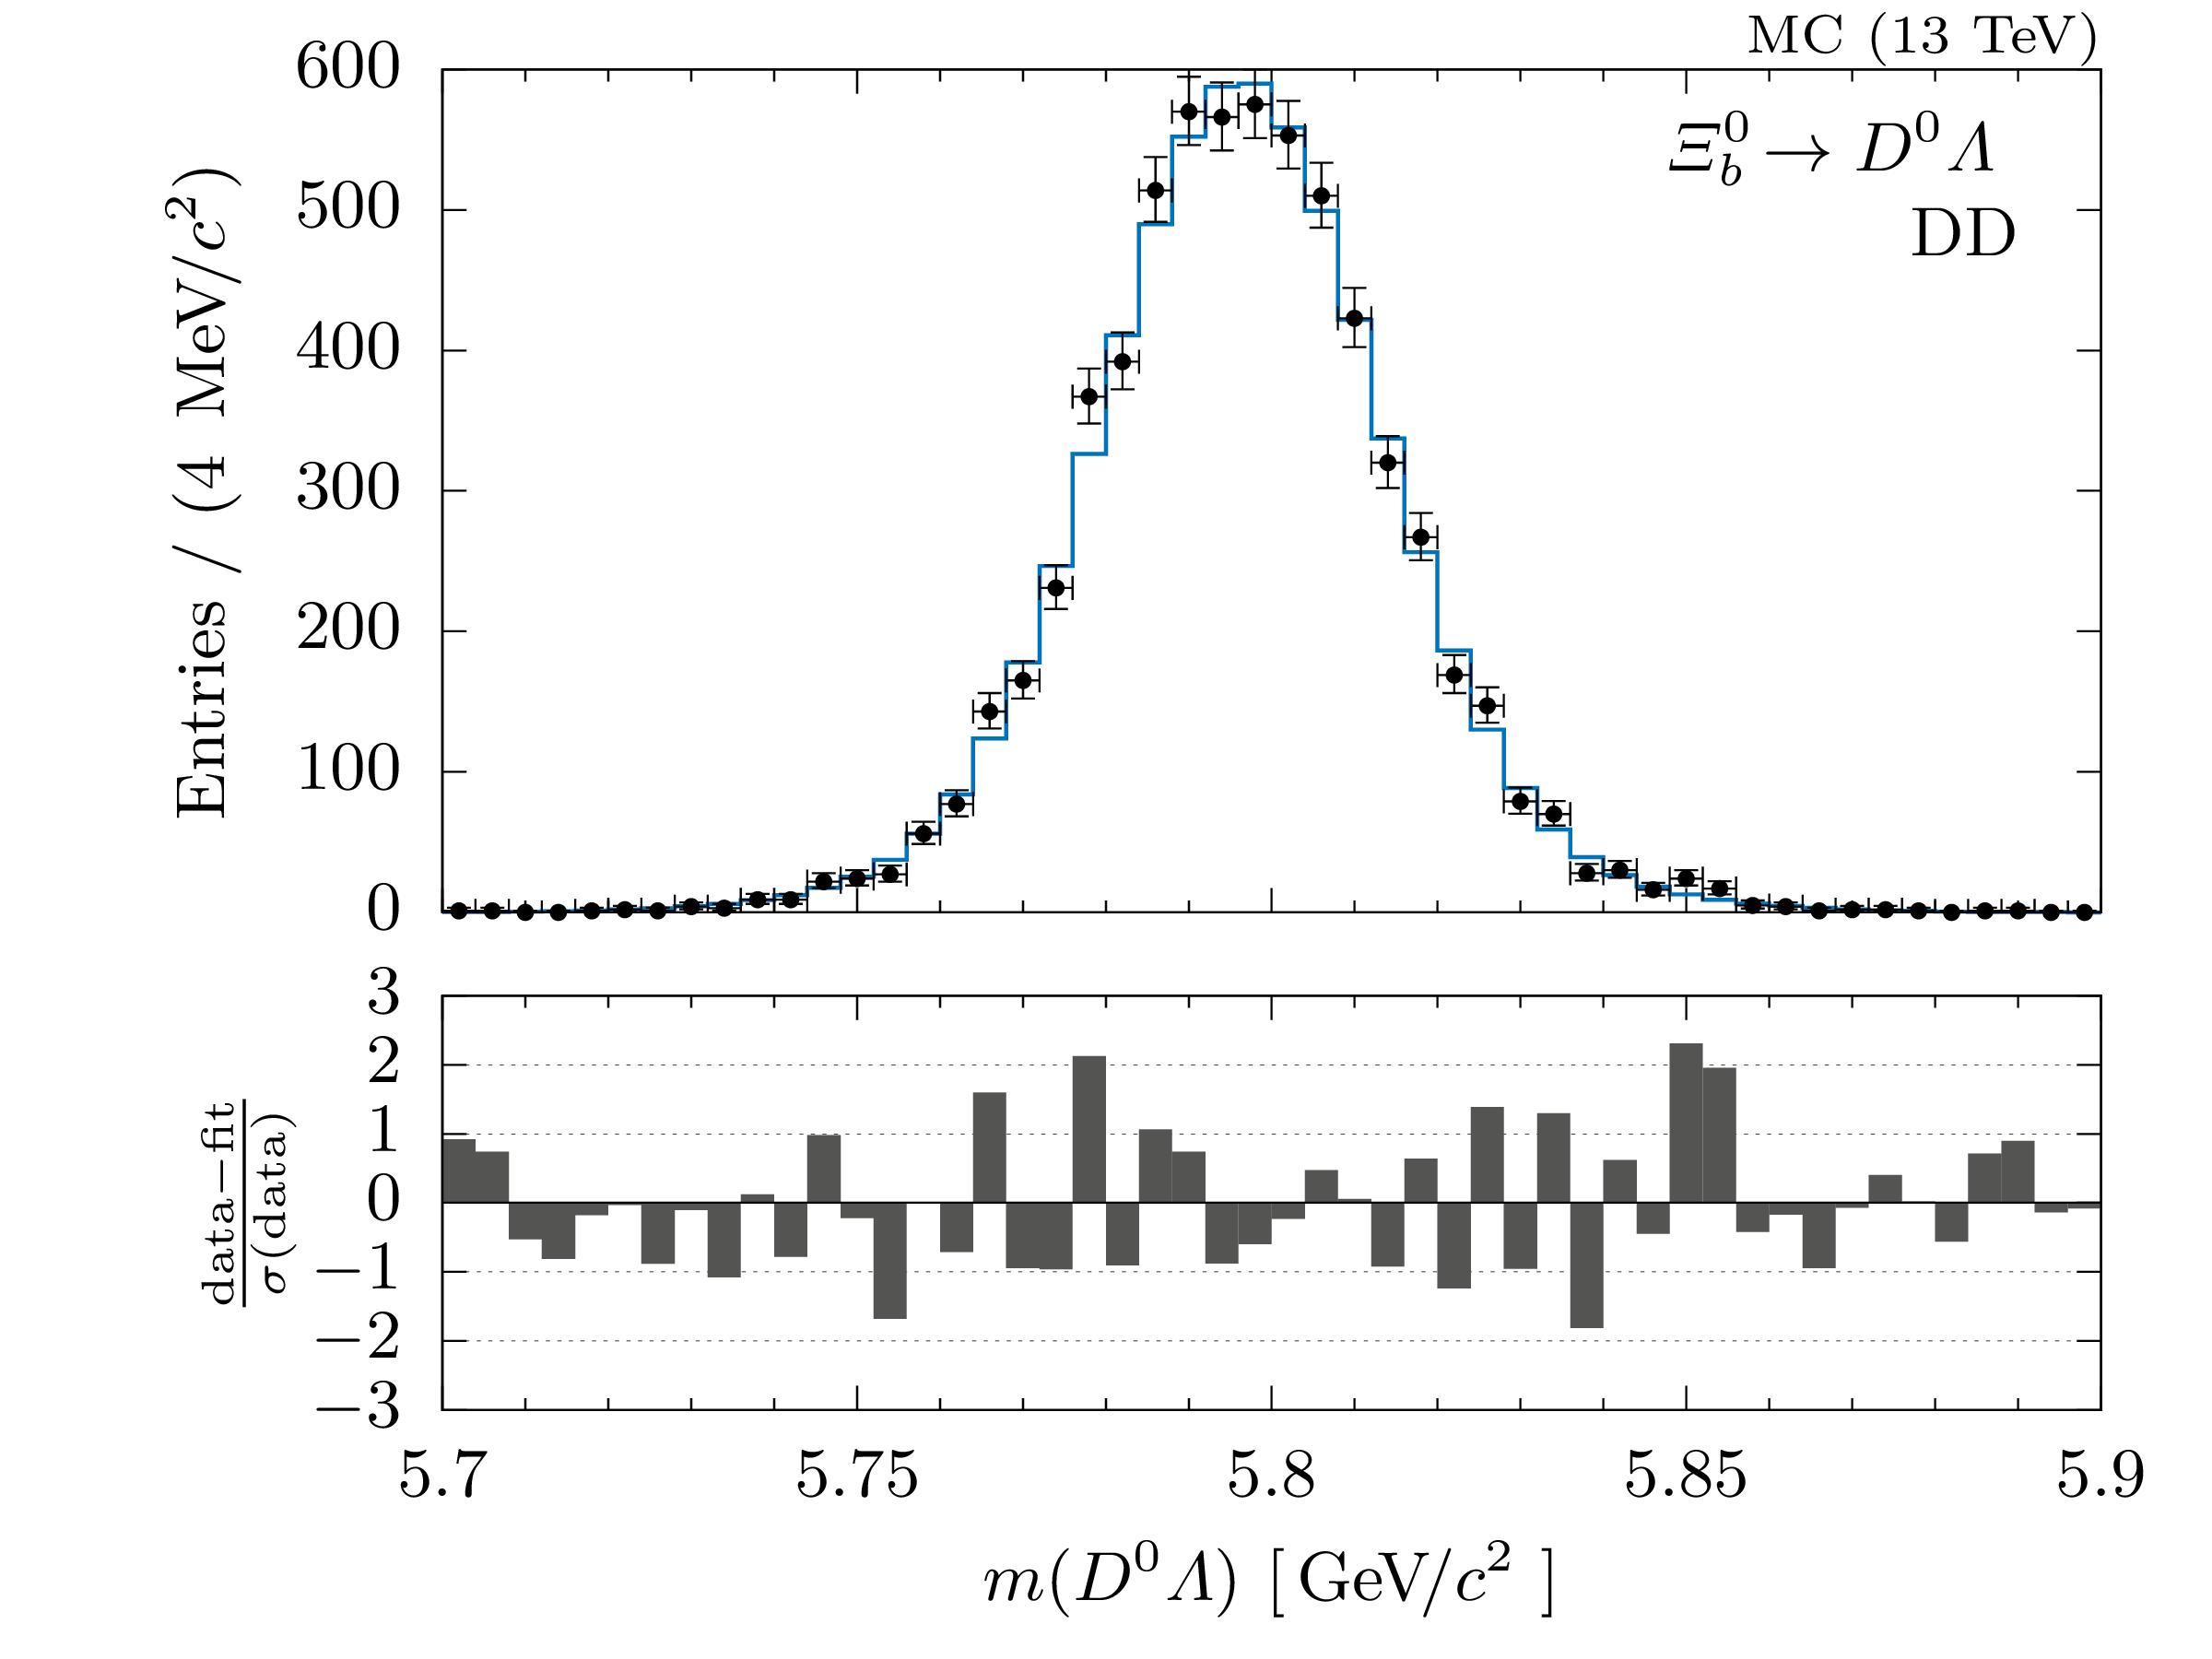
\includegraphics[scale=1.]{fit/hLbM_DD_MC_Xib.png}
    \end{subfigure}
    \caption{Combined invariant mass of \Dz and \Lz candidates of track type \gls{LL} (top) and \gls{DD} (bottom) from \gls{mc} simulated \decay{\Xibz}{\Dz\Lz} decays, as well as the corresponding projections of the simultaneous fit in configuration 1.}
    \label{fig:fit_hLbM_MC_Xib}
\end{figure}

\begin{figure}[htbp]
    \centering
    \begin{subfigure}[b]{\textwidth}
        \centering
        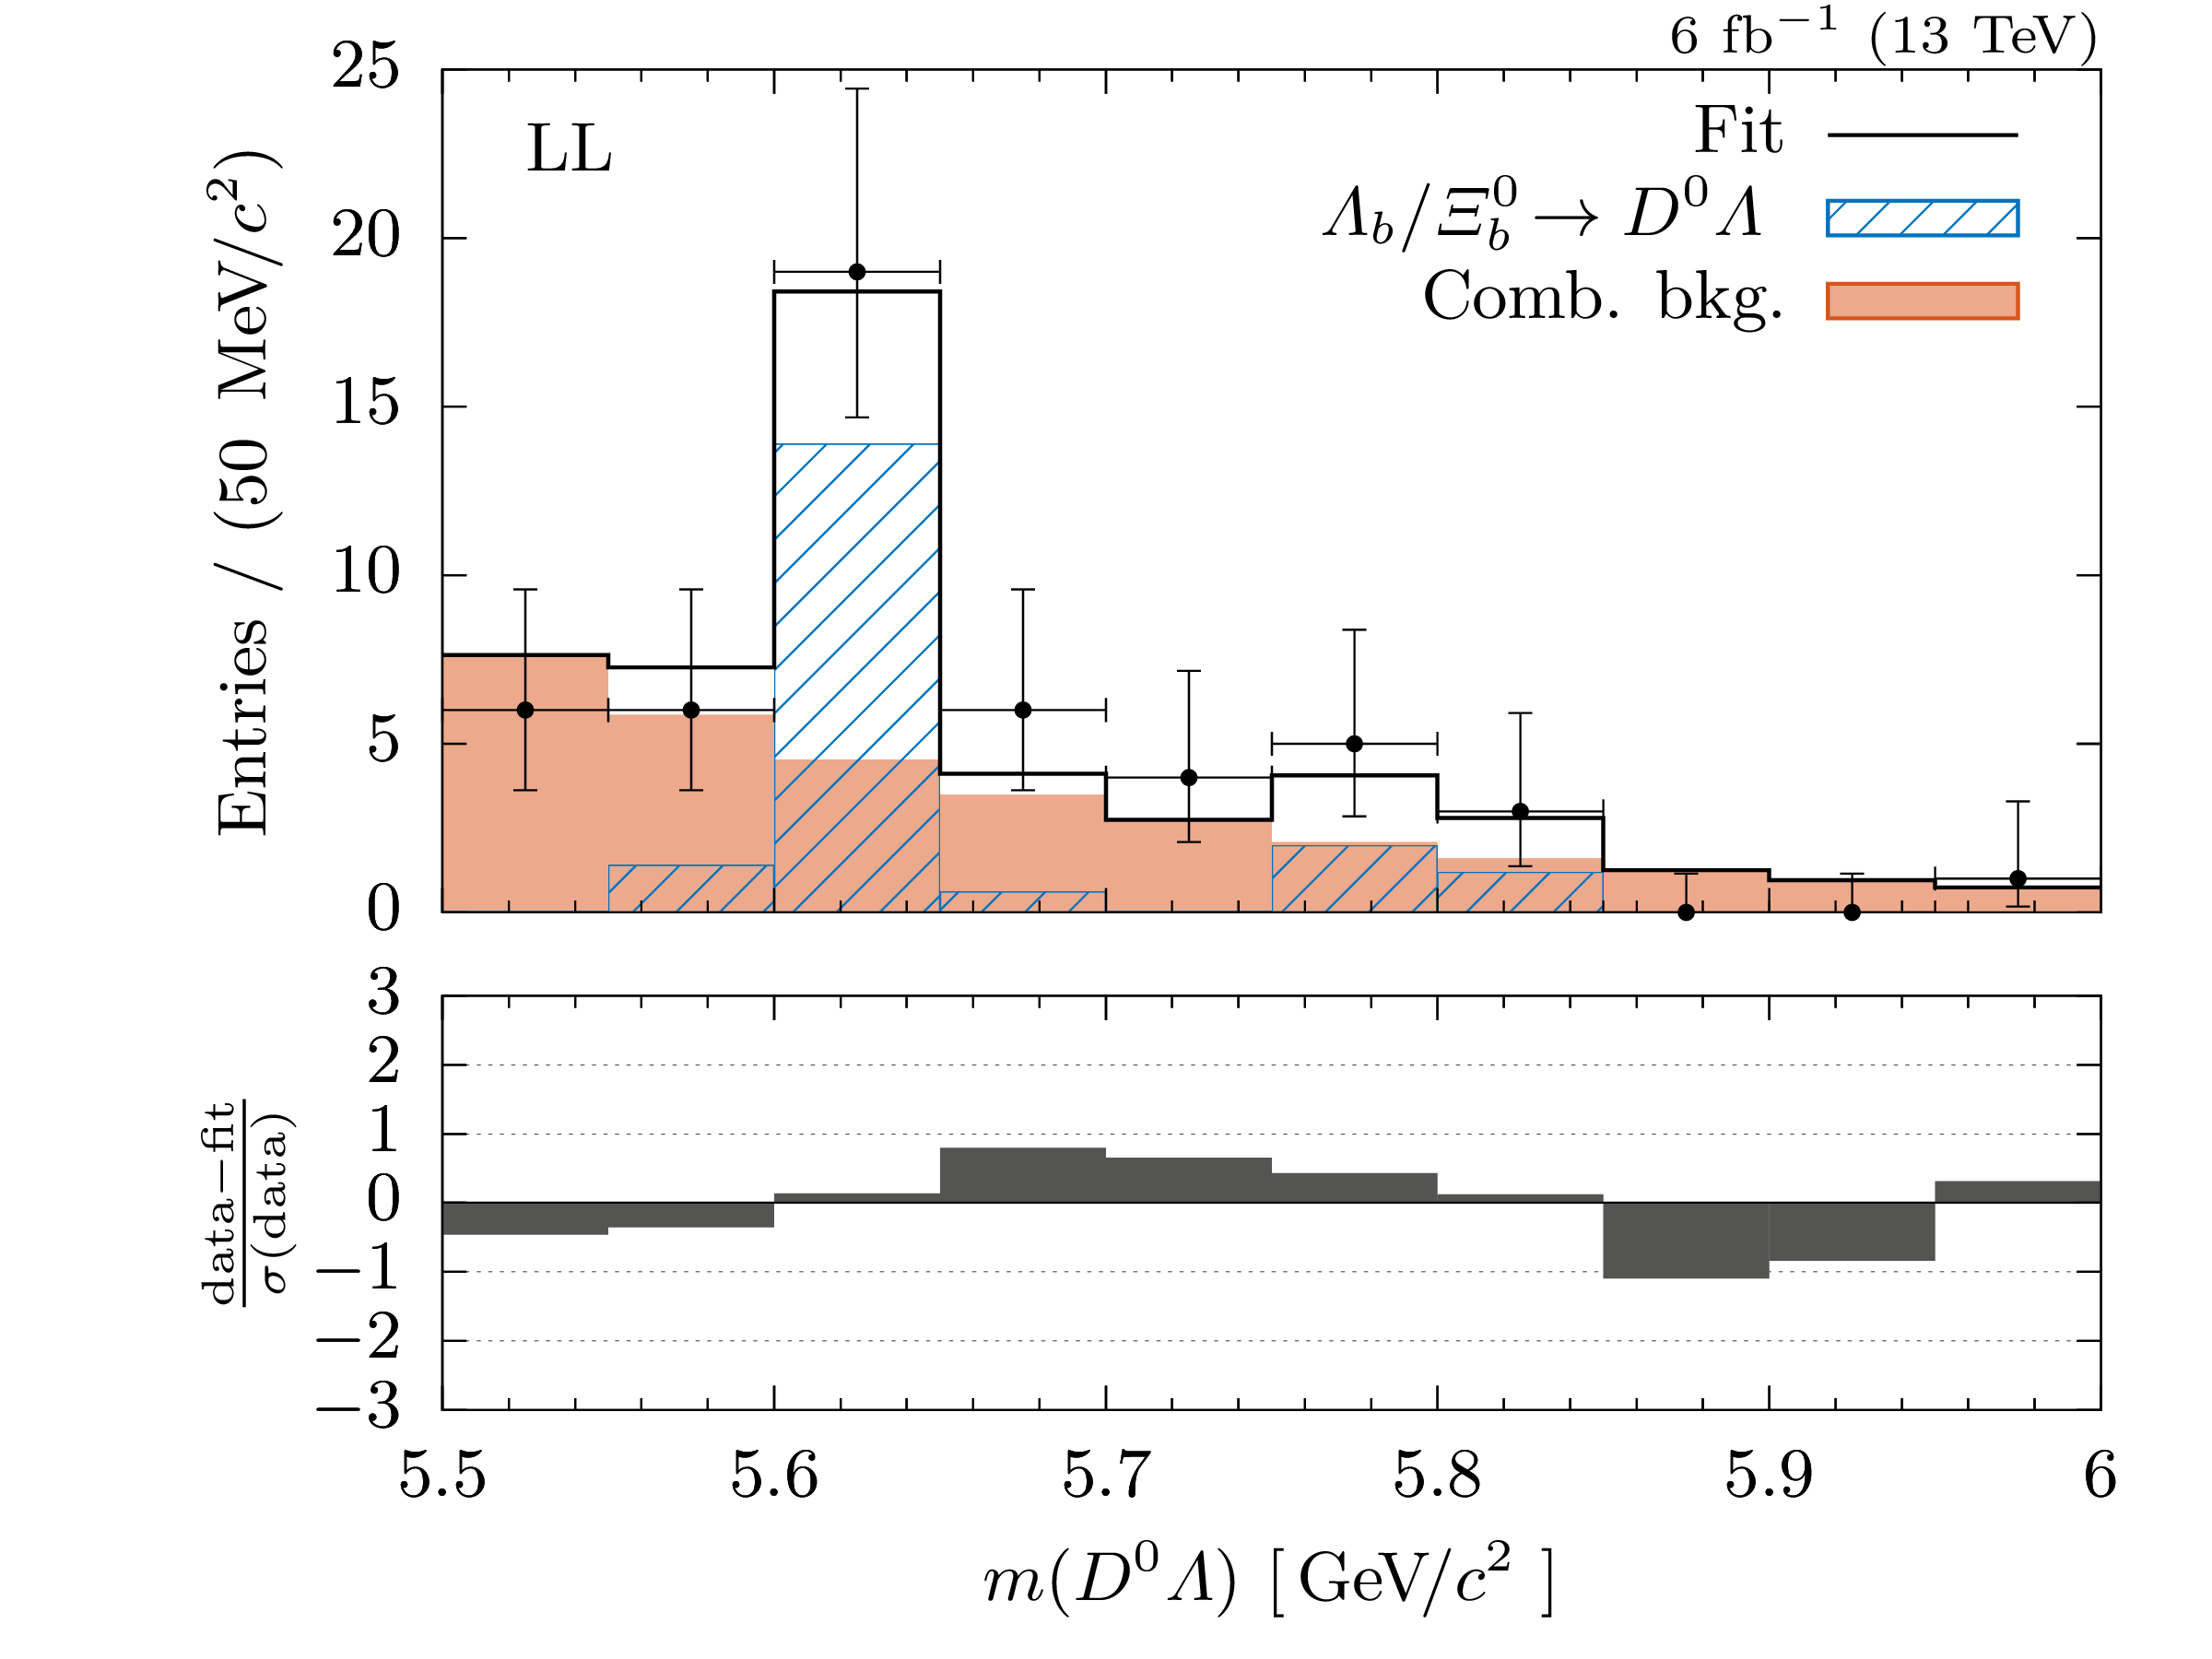
\includegraphics[scale=1.]{fit/hLbM_data_LL_fit1.png}
    \end{subfigure}
    \par\bigskip 
    \begin{subfigure}[b]{\textwidth}
        \centering
        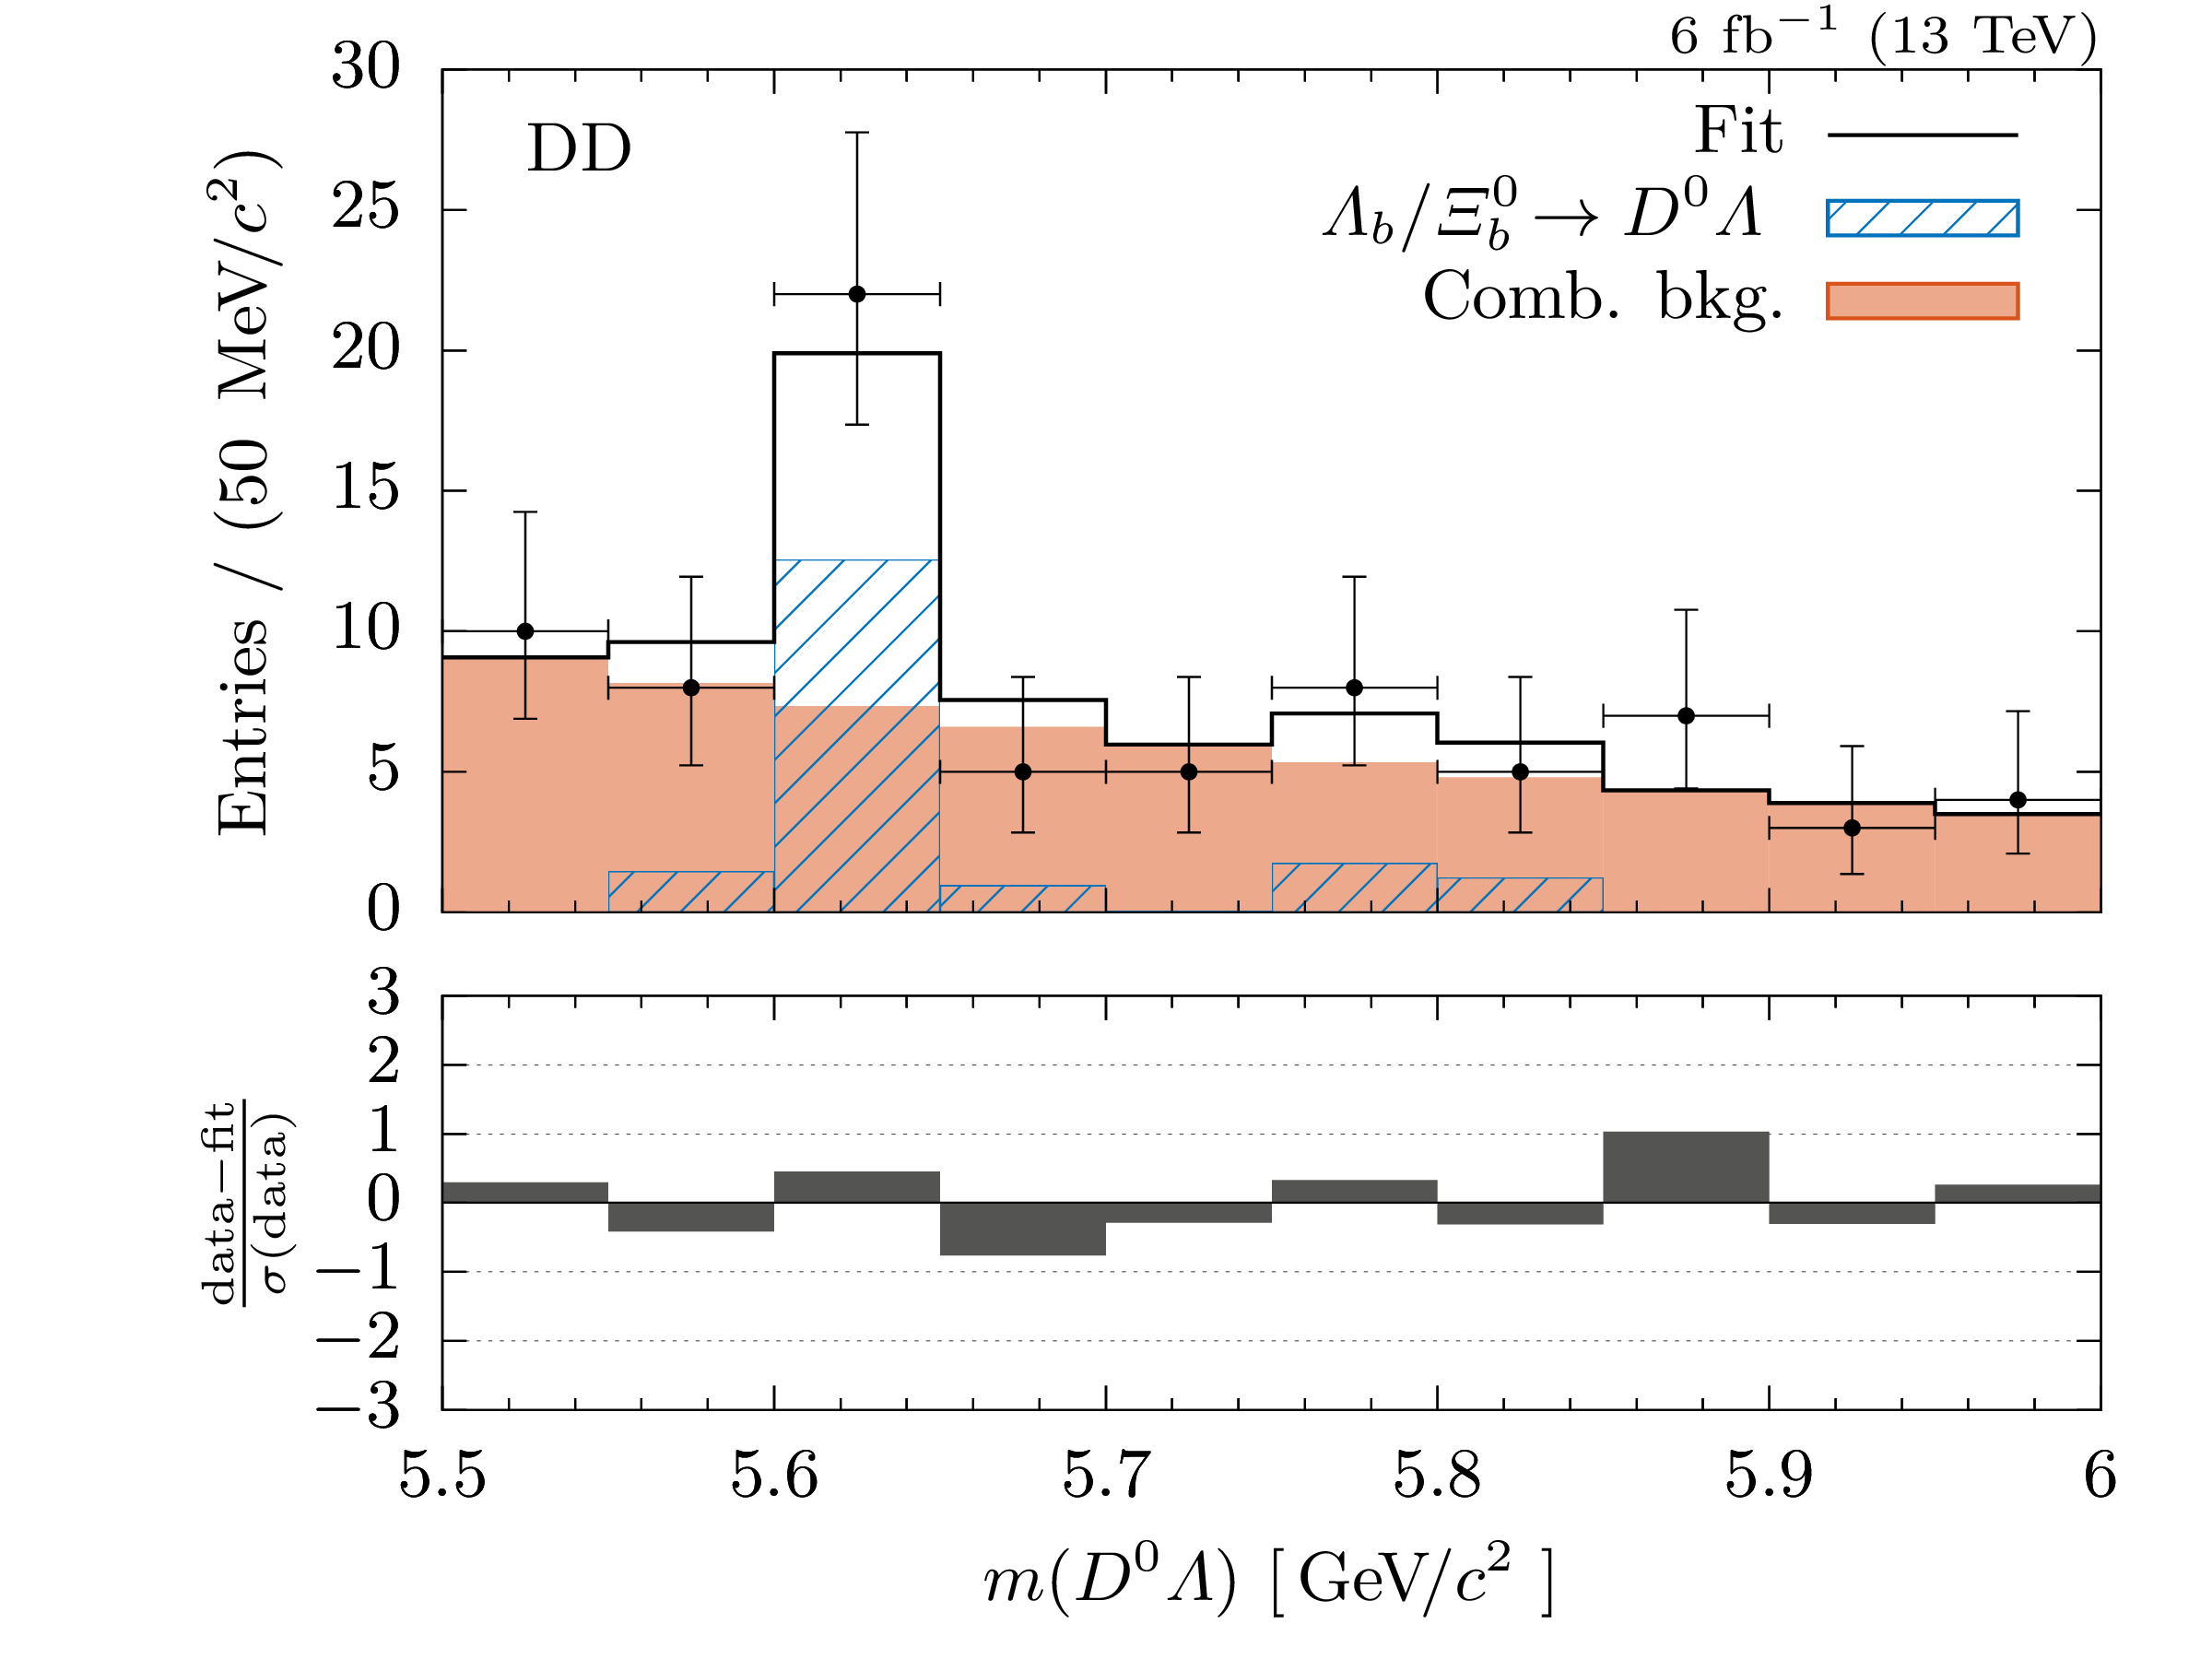
\includegraphics[scale=1.]{fit/hLbM_data_DD_fit1.png}
    \end{subfigure}
    \caption{Combined invariant mass of \Dz and \Lz candidates of track type \gls{LL} (top) and \gls{DD} (bottom) from recorded data, as well as the corresponding projections of the simultaneous fit in configuration 1.}
    \label{fig:fit_hLbM_data_fit1_LLDD}
\end{figure}

\begin{figure}[htbp]
    \centering
    \begin{subfigure}[b]{\textwidth}
        \centering
        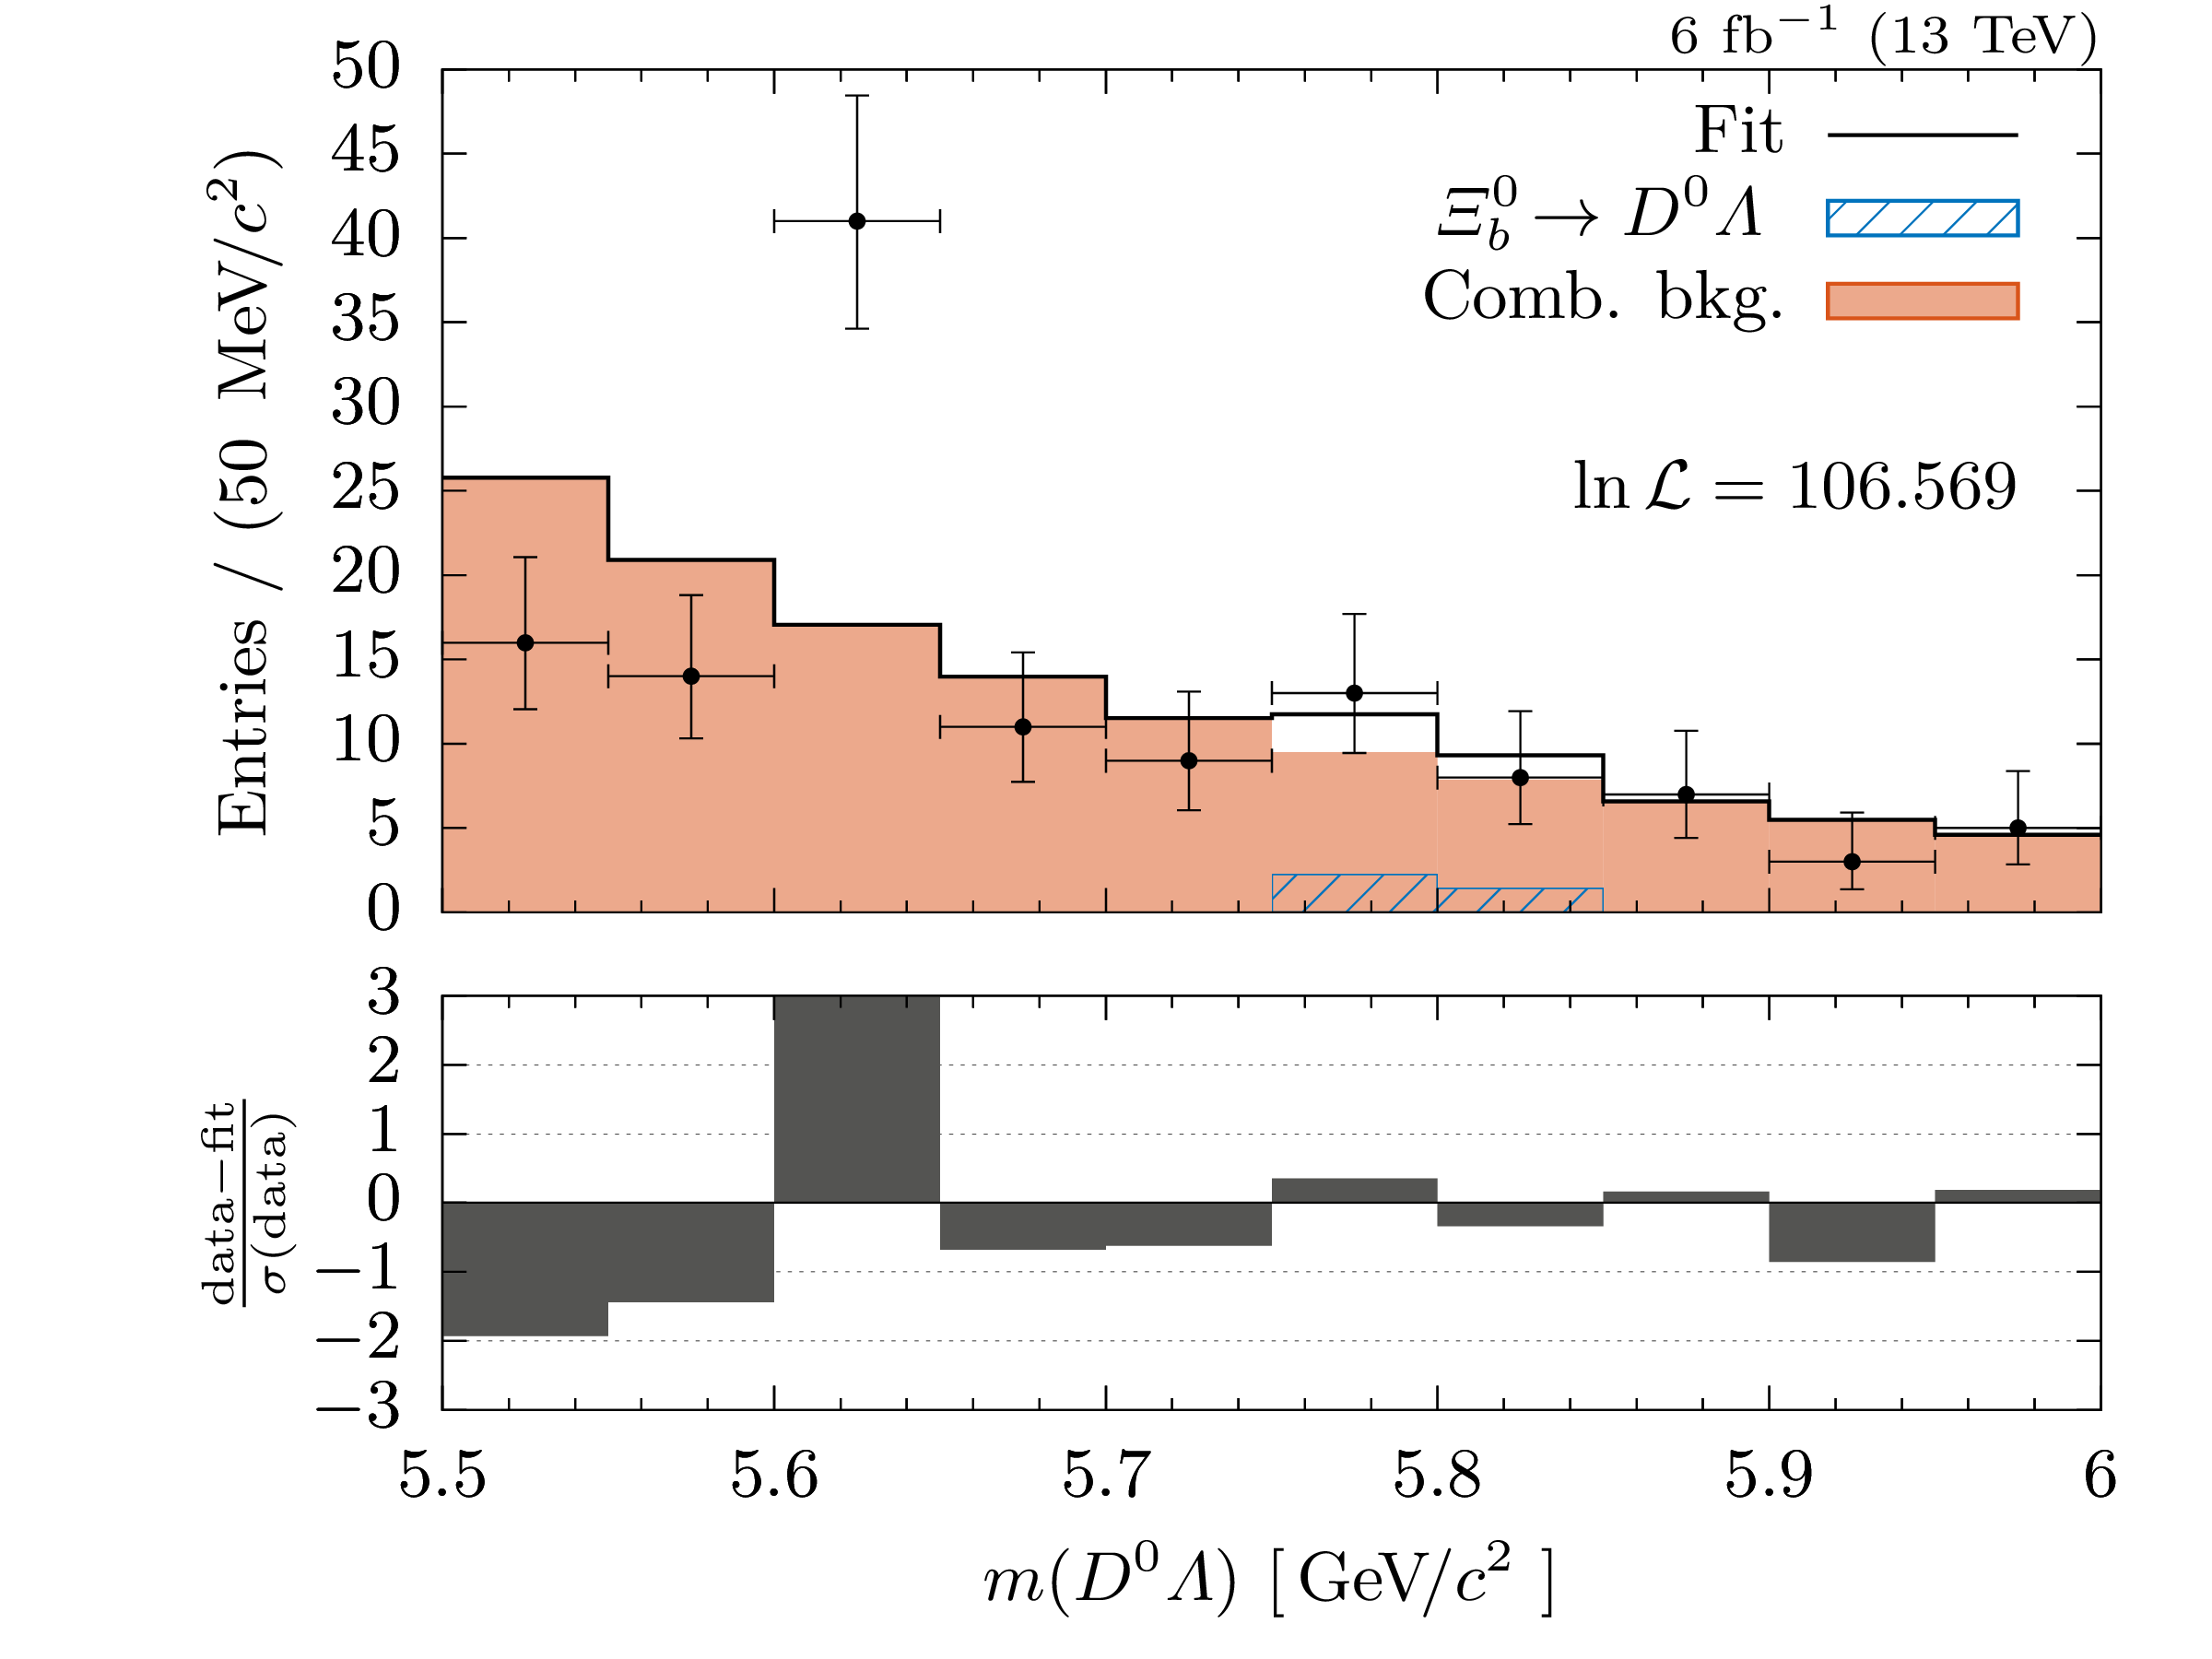
\includegraphics[scale=1.]{fit/hLbM_data_fit2_2.png}
    \end{subfigure}
    \par\bigskip 
    \begin{subfigure}[b]{\textwidth}
        \centering
        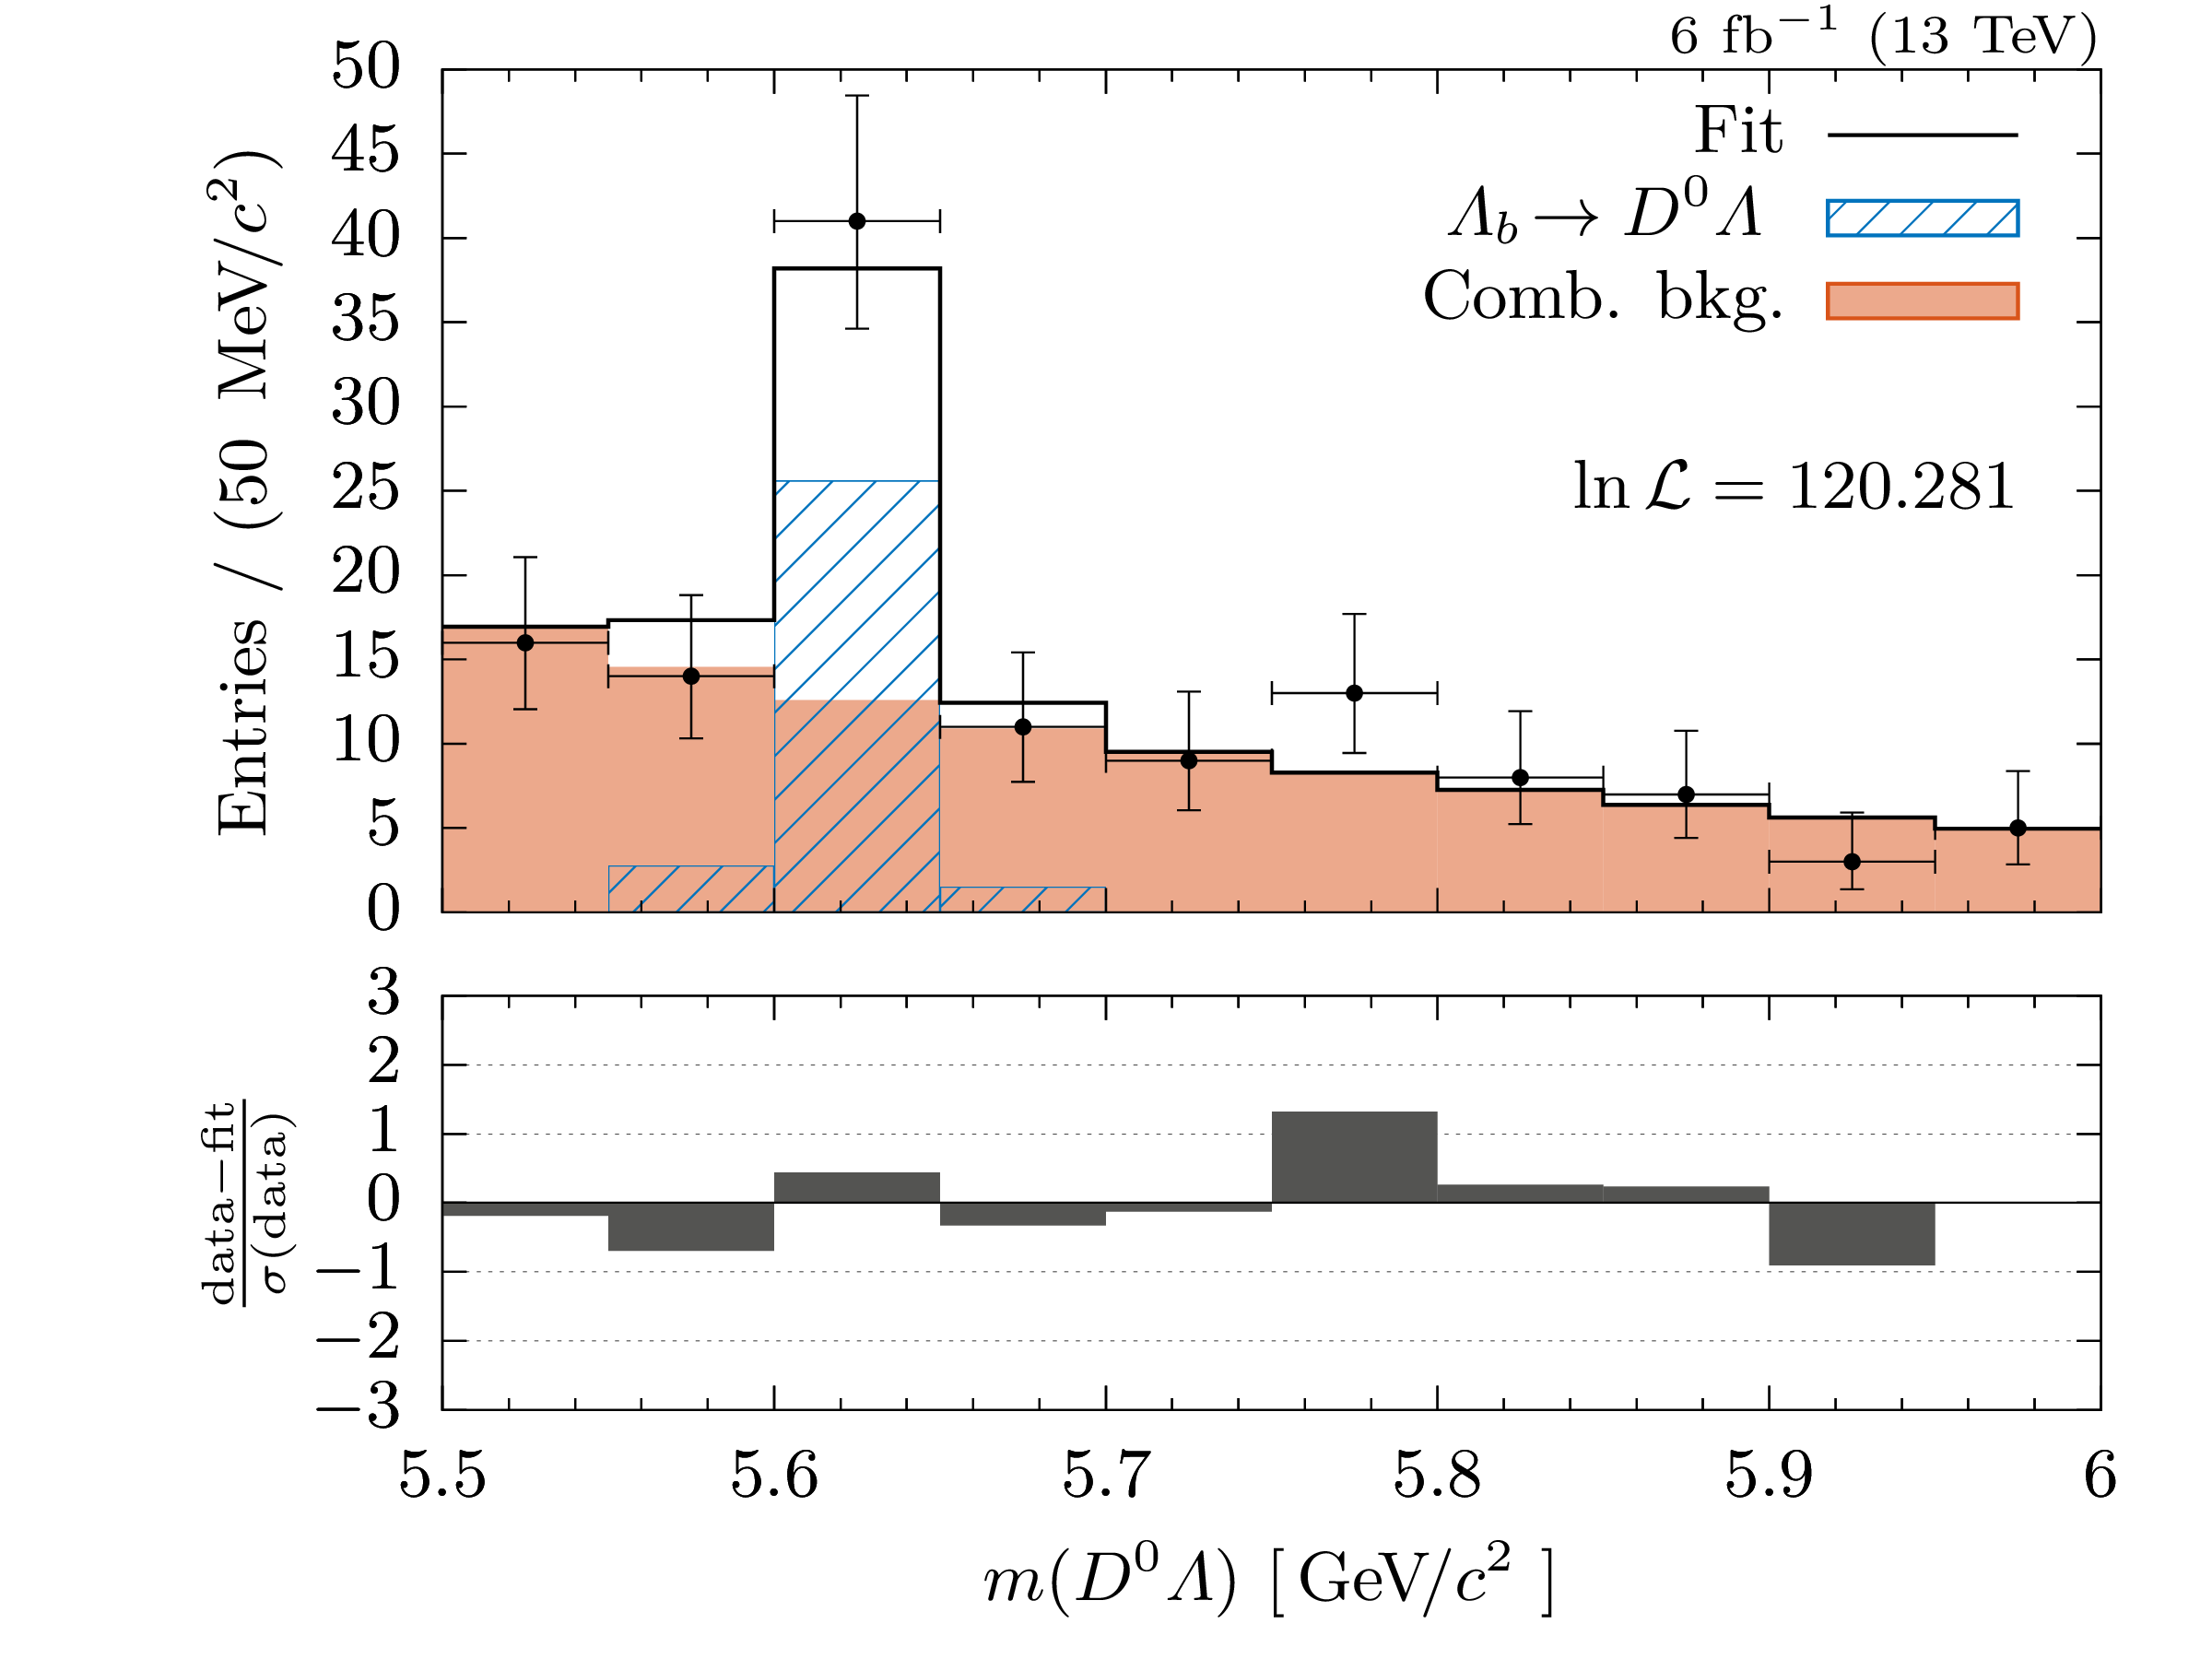
\includegraphics[scale=1.]{fit/hLbM_data_fit2_3.png}
    \end{subfigure}
    \caption{Combined invariant mass of \Dz and \Lz candidates from recorded data, as well as the corresponding accumulated projections of the simultaneous fit for both track types. These fits are used to extract the yield significance of \decay{\Lb}{\Dz\Lz} (top) and \decay{\Xibz}{\Dz\Lz} (bottom). The log-likelihood when both modes are enabled (one \gls{dof} more) is $\ln \mathcal{L} = 121.944$.}
    \label{fig:fit_hLbM_data_fit23}
\end{figure}

\begin{figure}[htbp]
    \centering
    \begin{subfigure}[b]{\textwidth}
        \centering
        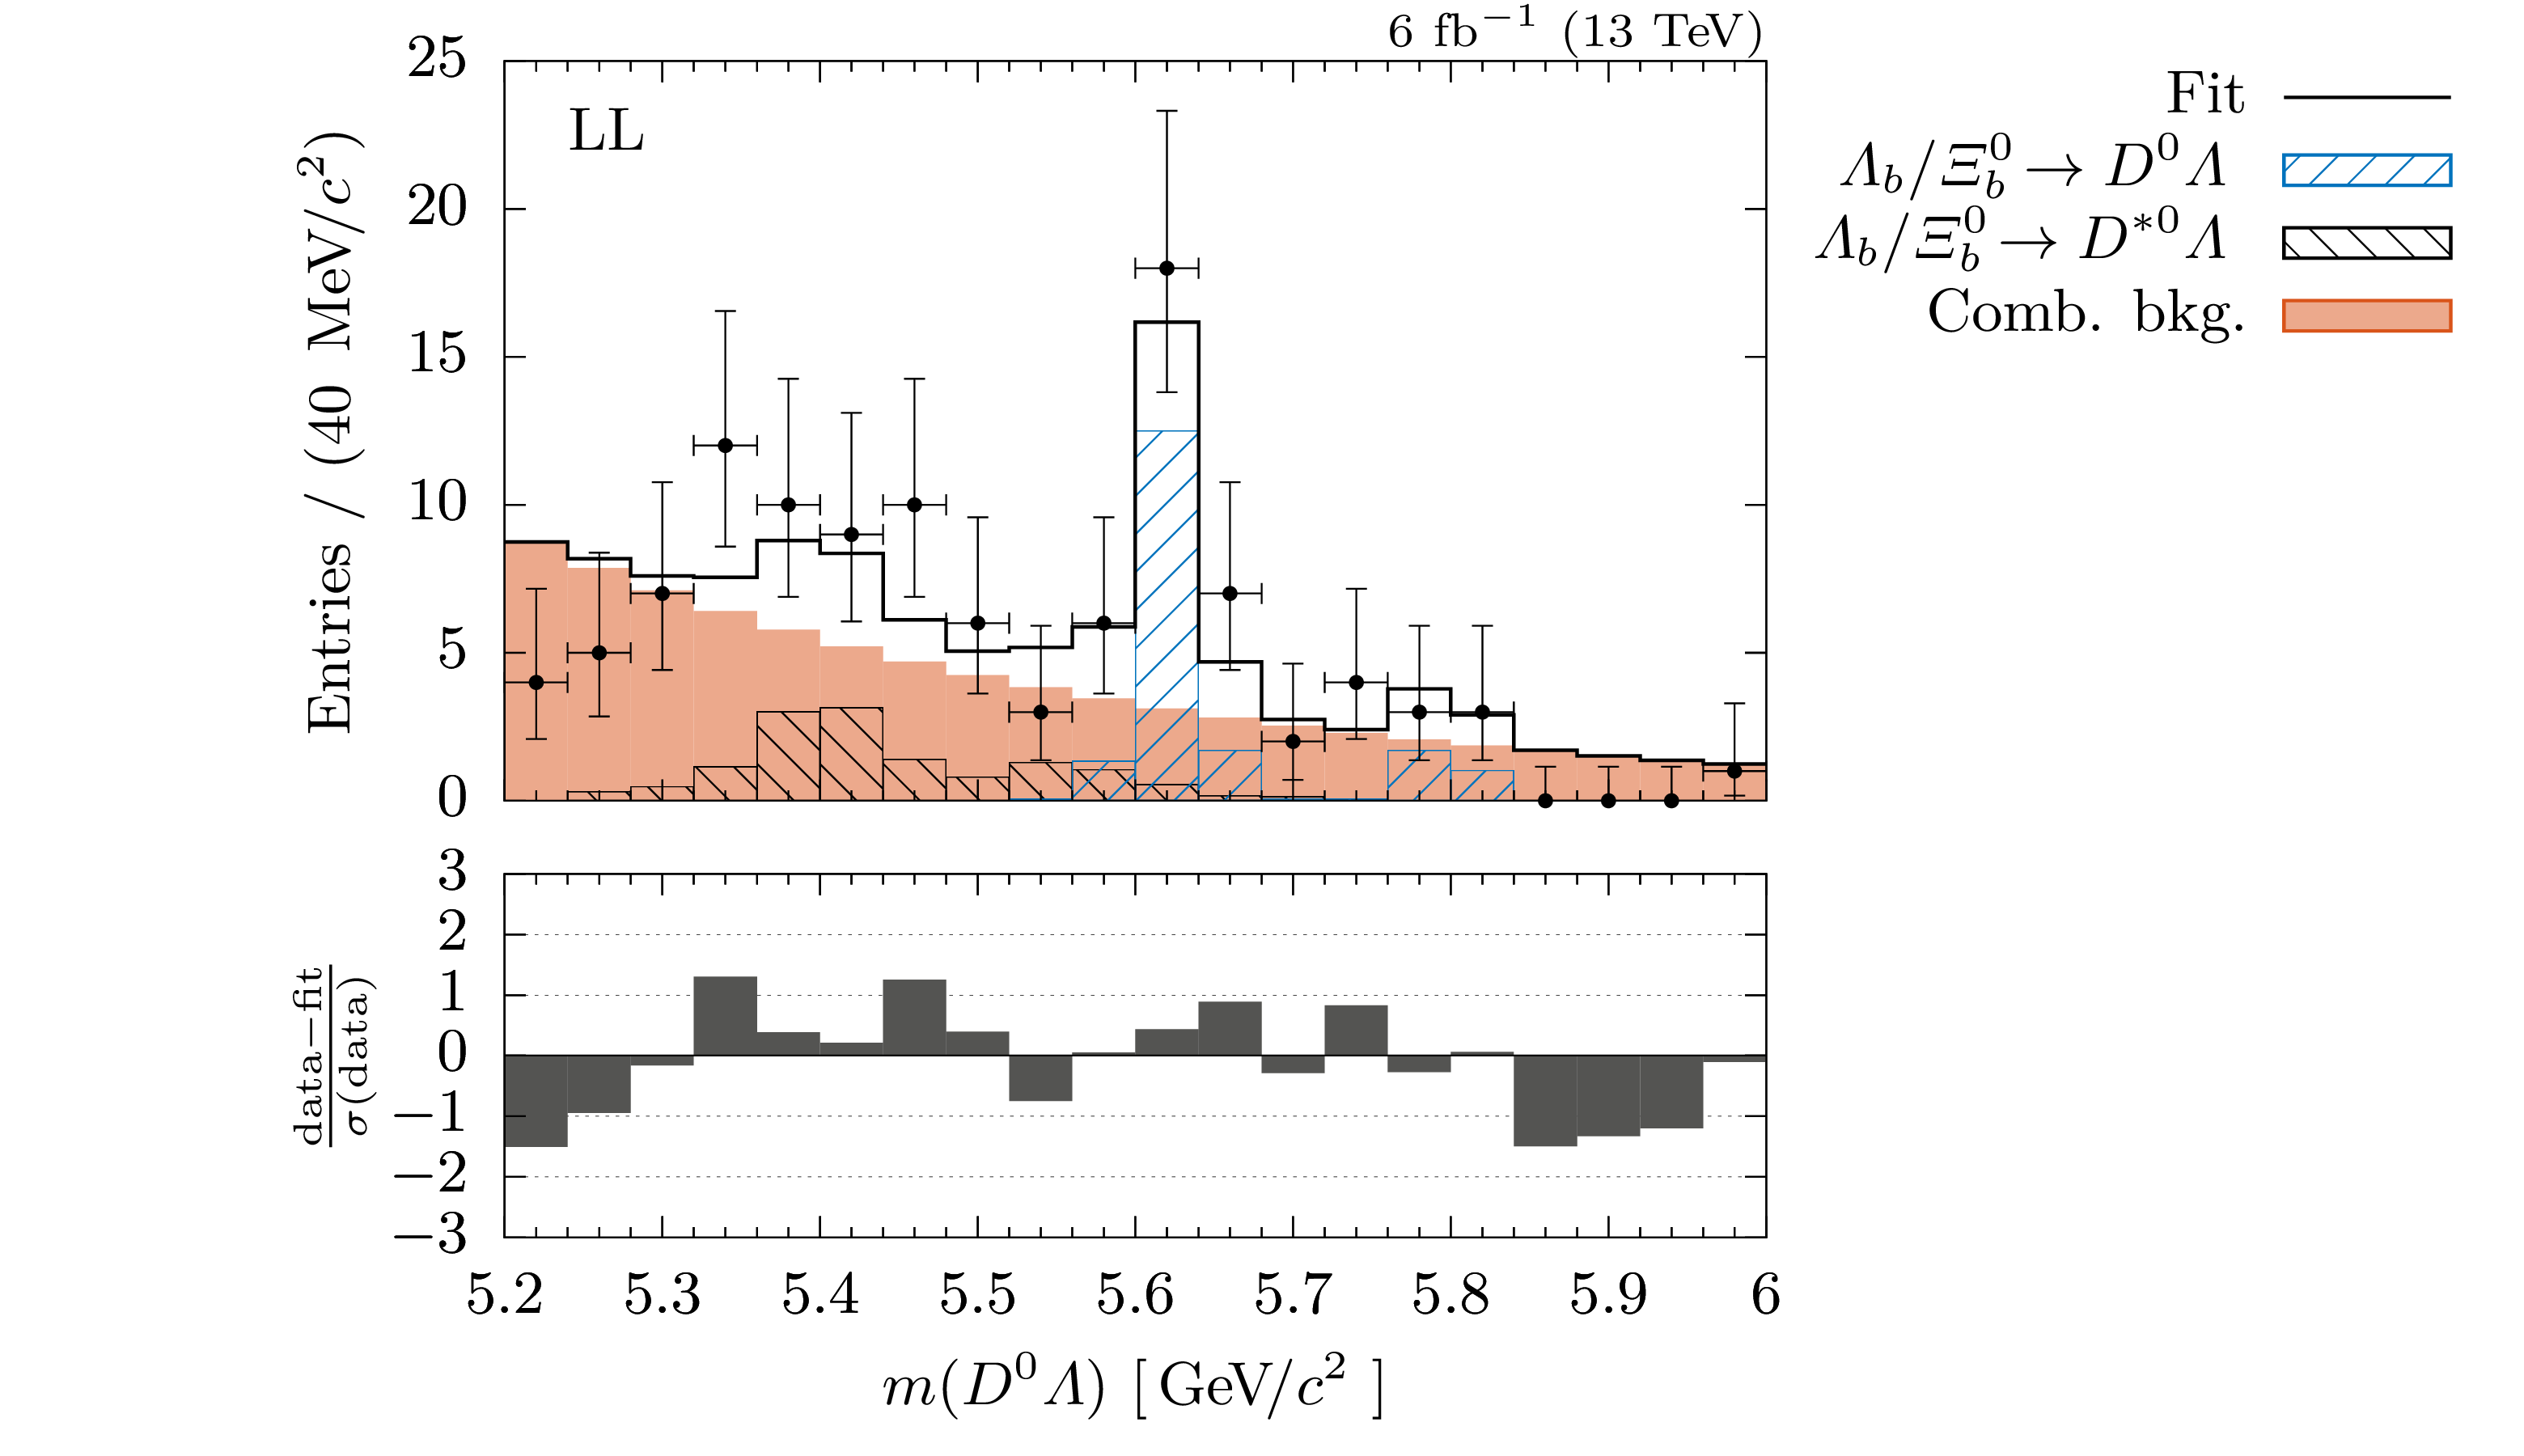
\includegraphics[scale=1.]{fit/hLbM_data_LL_fit3.png}
    \end{subfigure}
    \par\bigskip 
    \begin{subfigure}[b]{\textwidth}
        \centering
        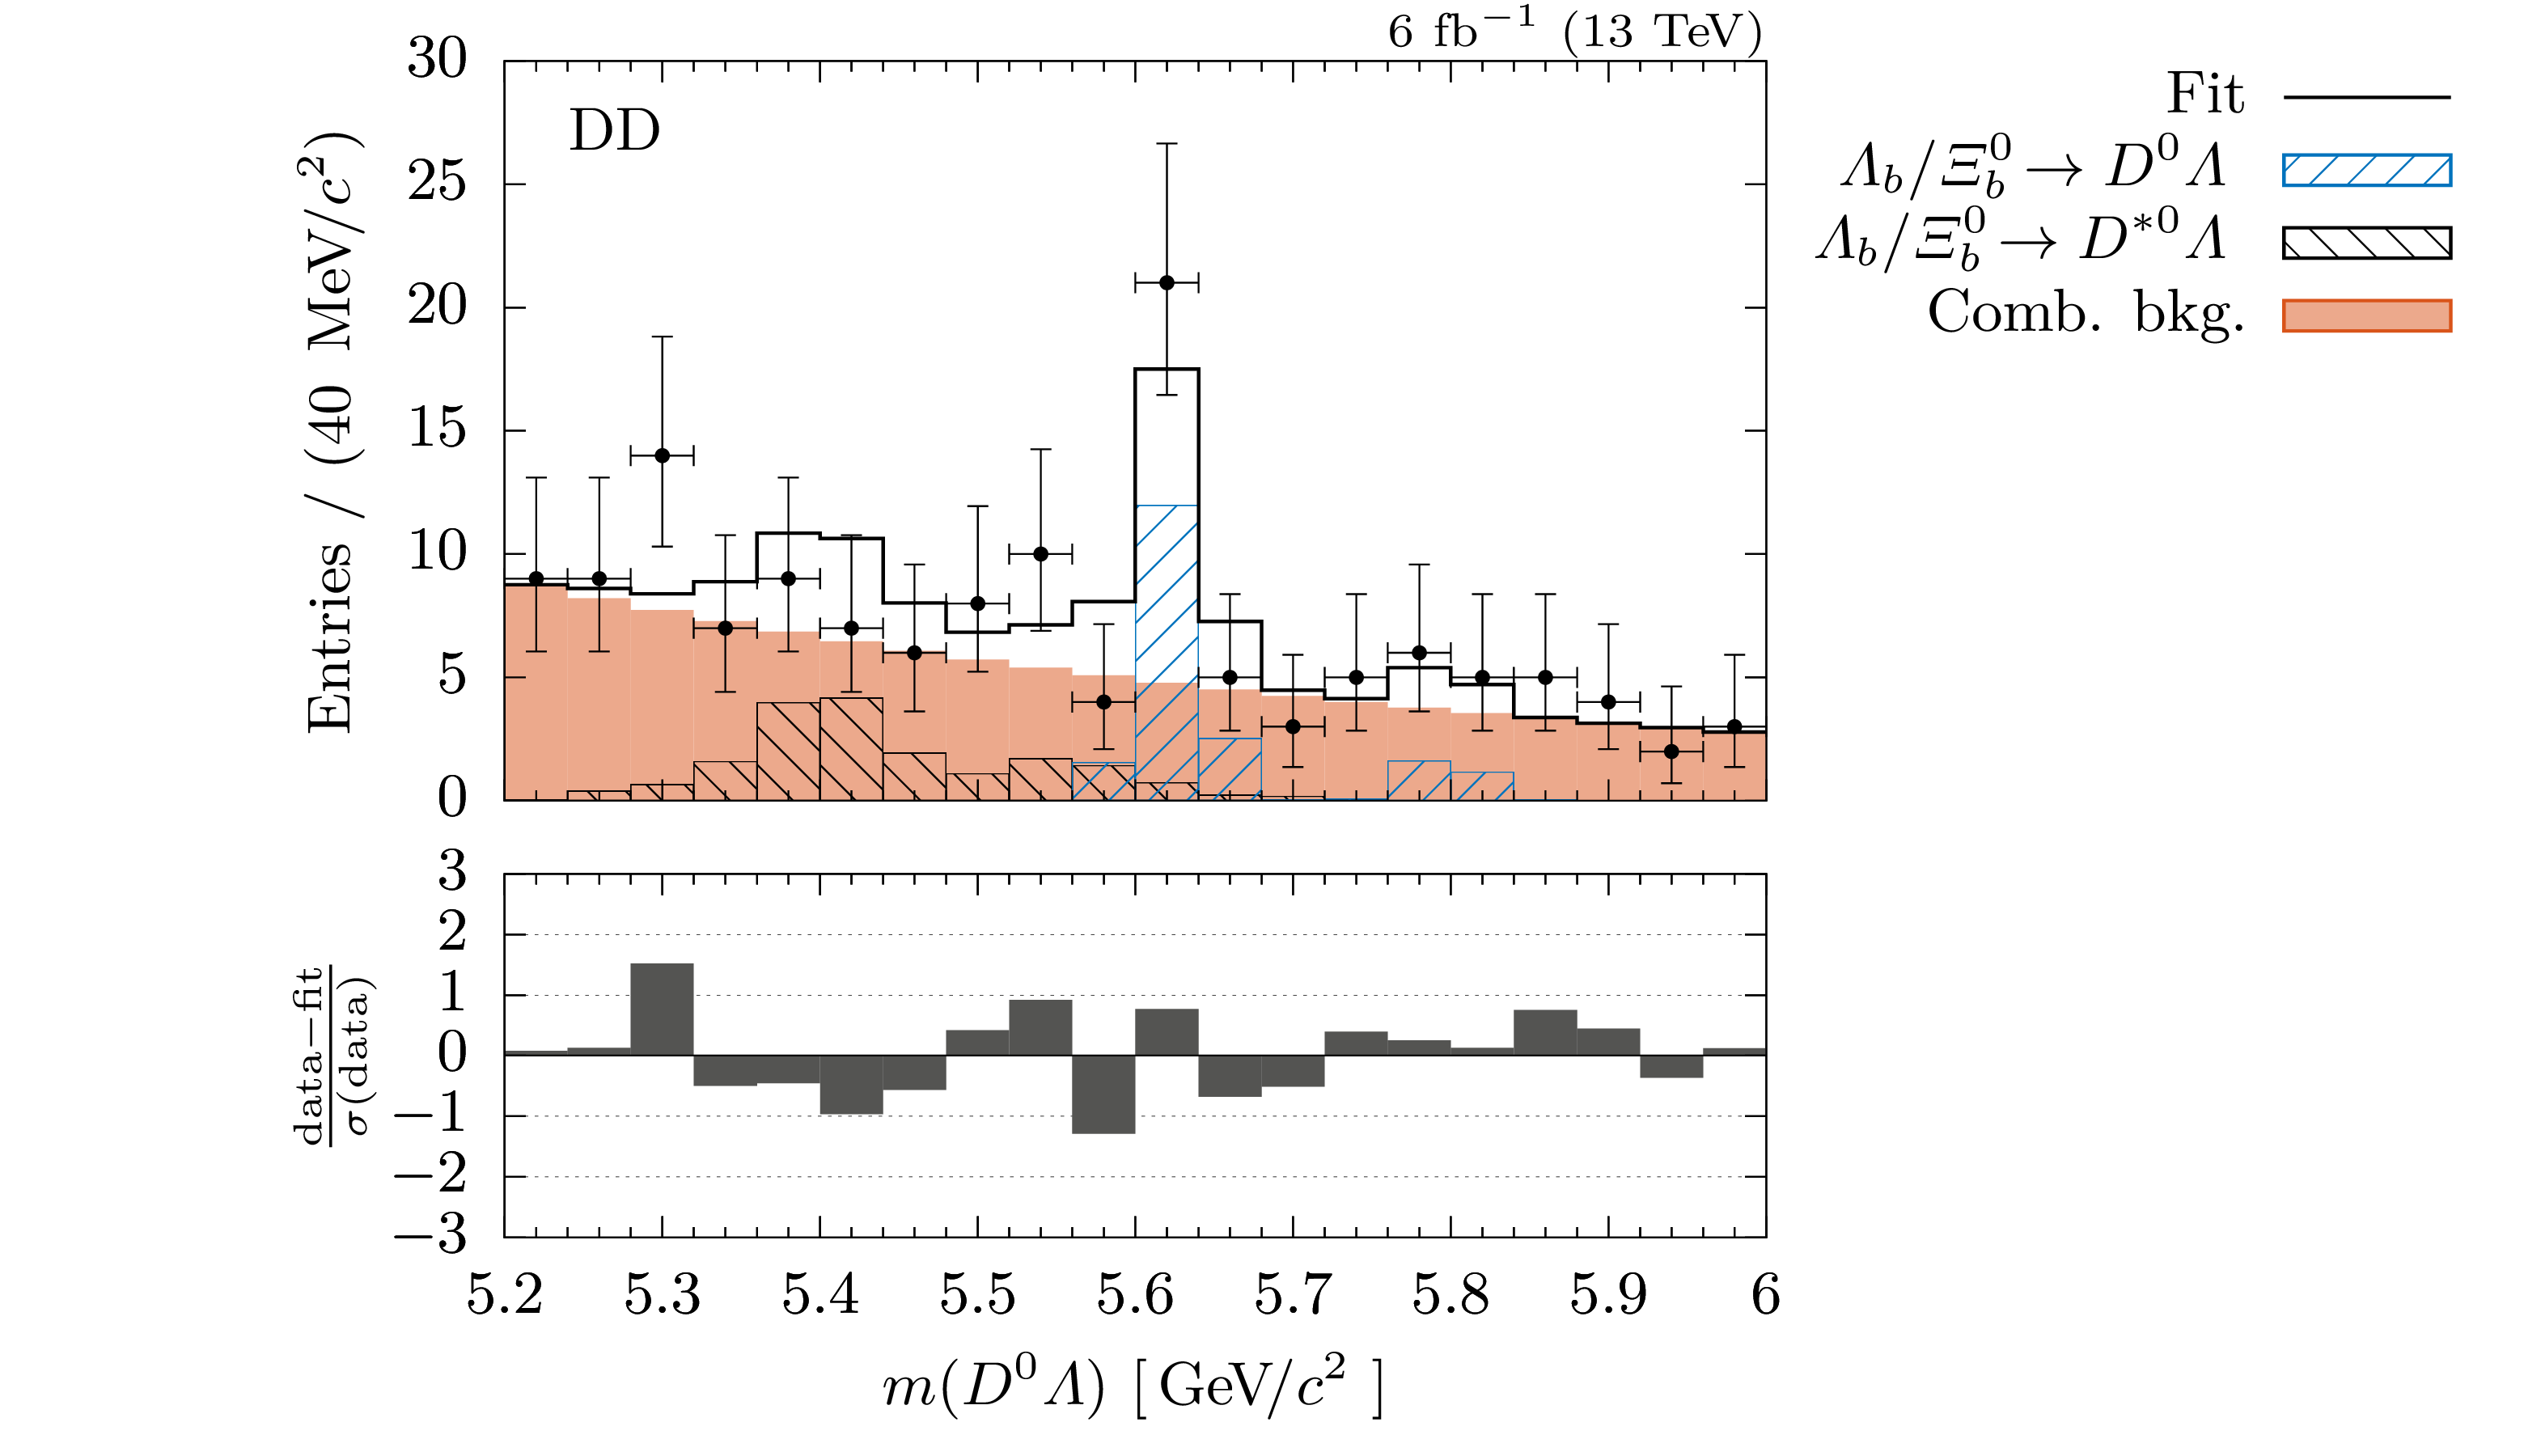
\includegraphics[scale=1.]{fit/hLbM_data_DD_fit3.png}
    \end{subfigure}
    \caption{Combined invariant mass of \Dz and \Lz candidates of track type \gls{LL} (top) and \gls{DD} (bottom), as well as the corresponding projections of the fit in configuration 3. The yield of the \Dstarz background is constrained among both track types, presumably causing the overshooting of the combinatorial background in the former mode.}
    \label{fig:fit_hLbM_data_fit3}
\end{figure}

\begin{figure}[htbp]
    \centering
    \begin{subfigure}[b]{\textwidth}
        \centering
        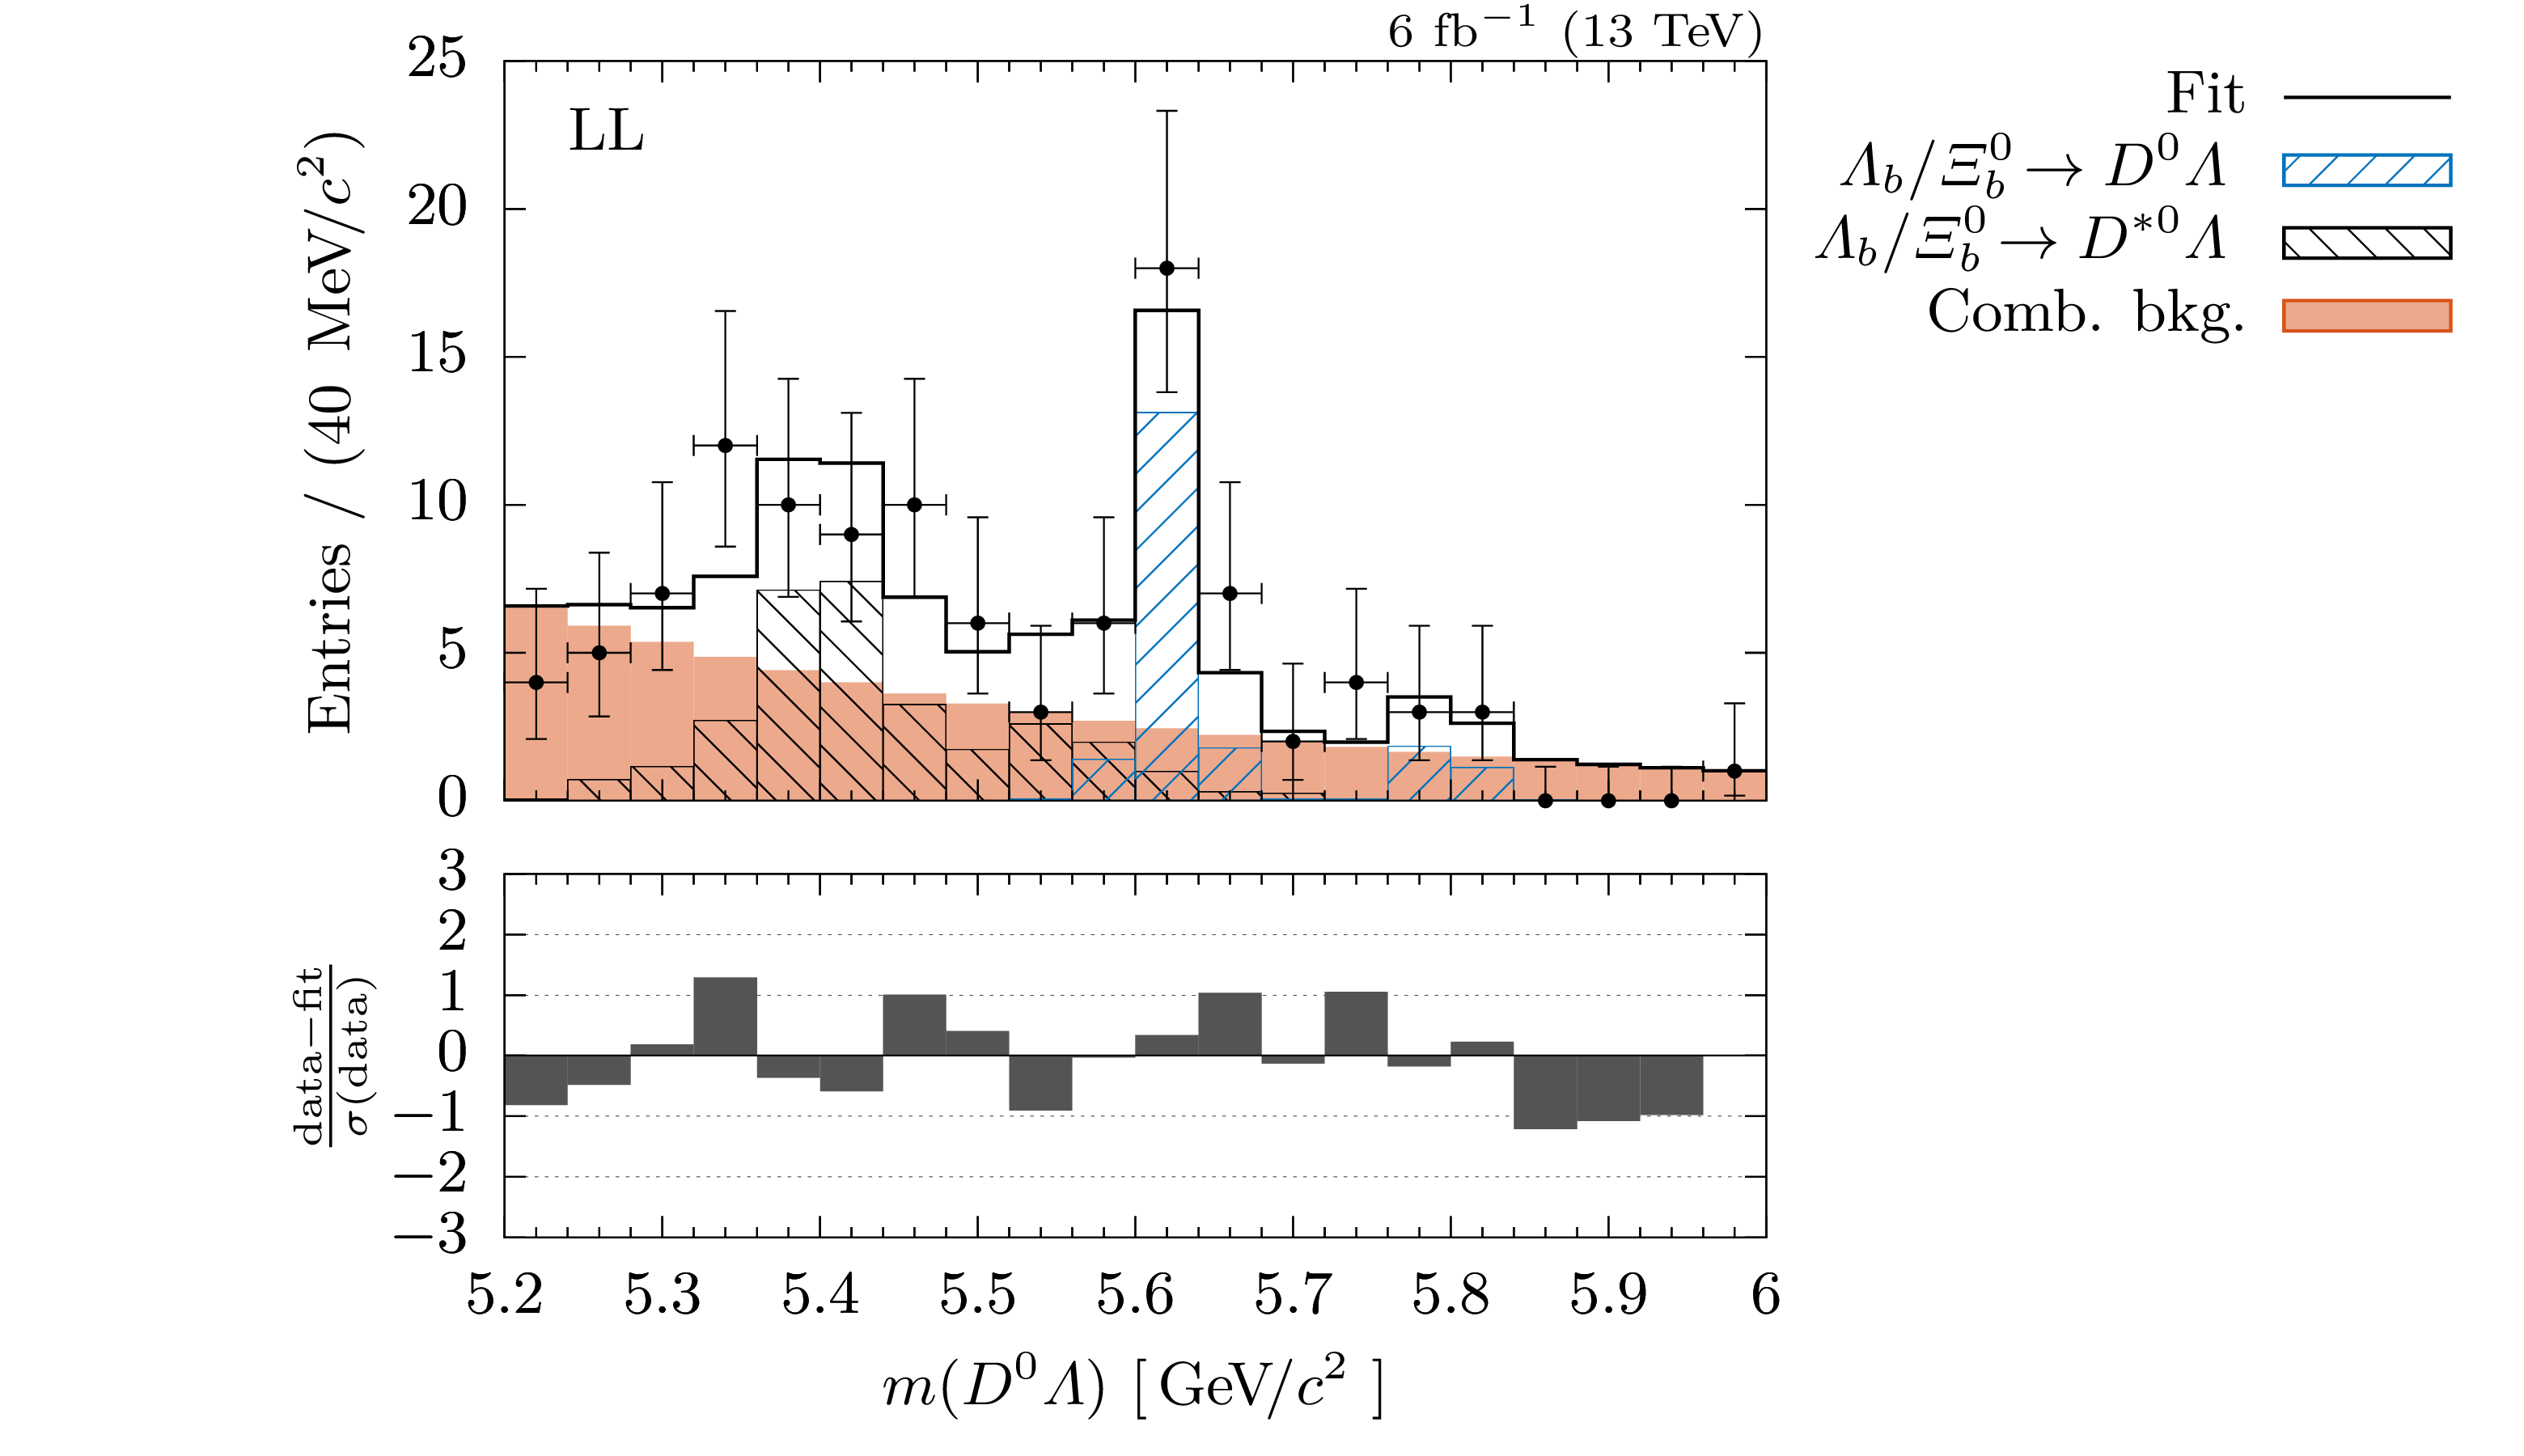
\includegraphics[scale=1.]{fit/hLbM_data_LL_fit4.png}
    \end{subfigure}
    \par\bigskip 
    \begin{subfigure}[b]{\textwidth}
        \centering
        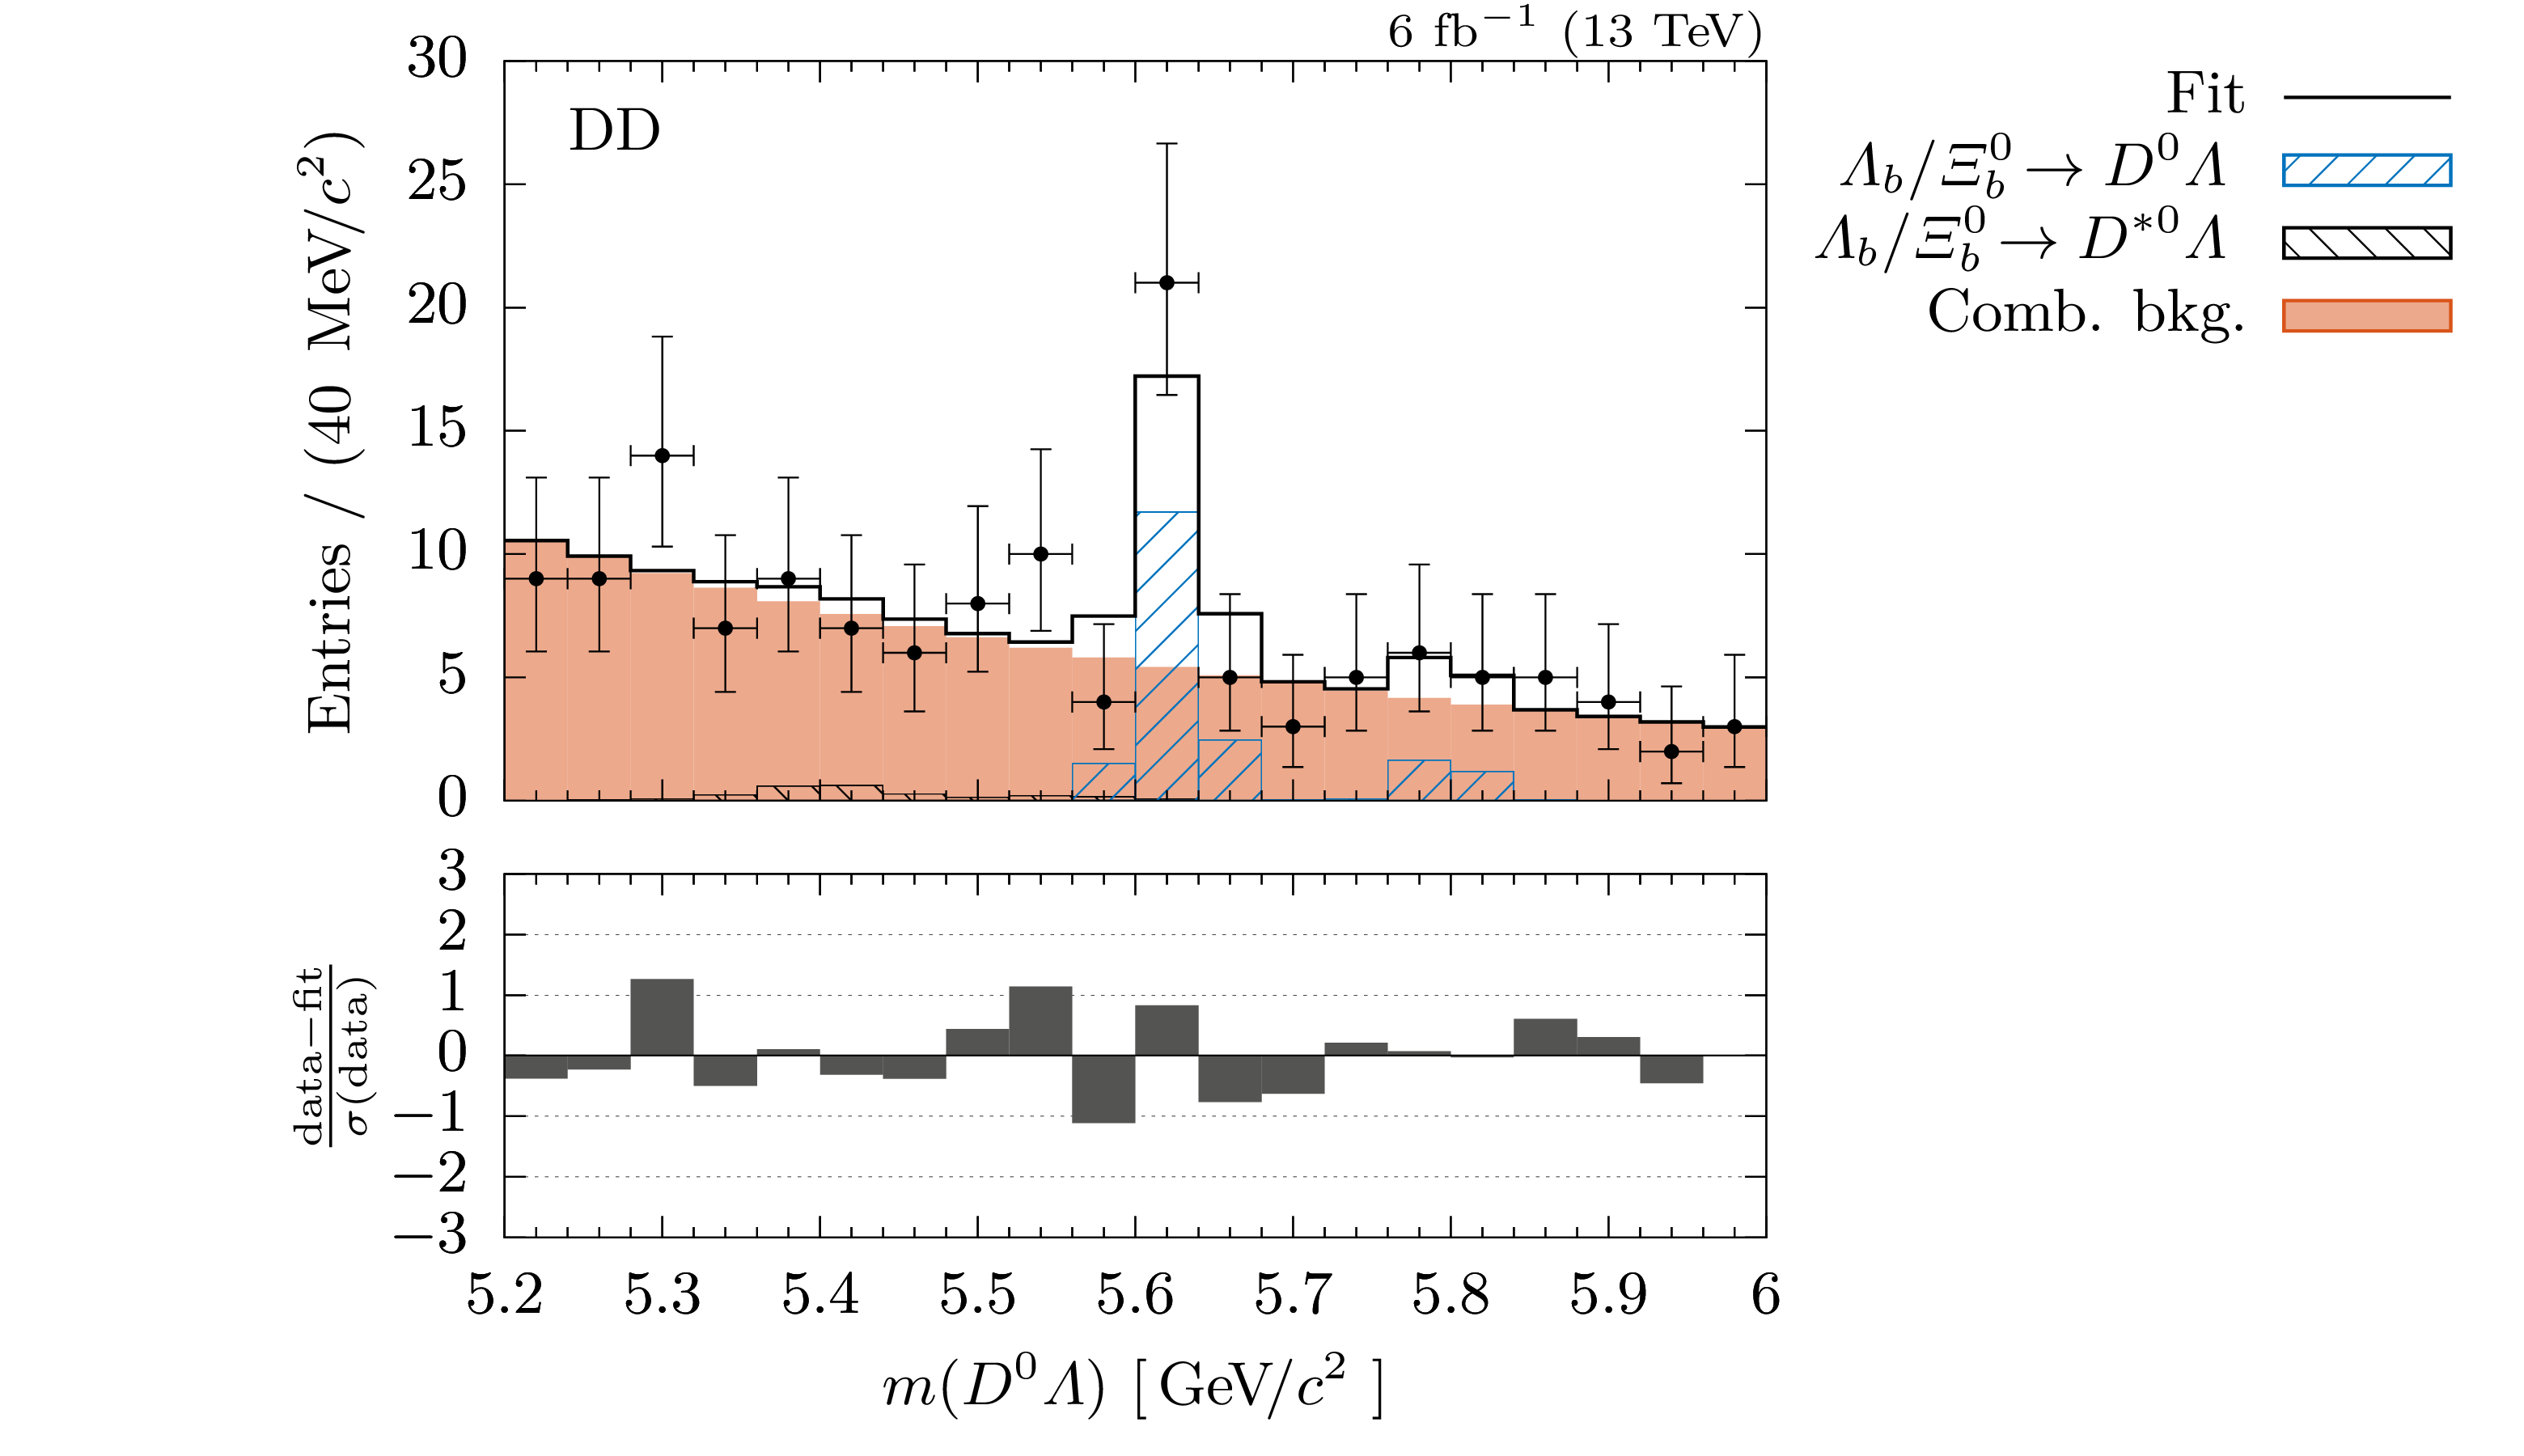
\includegraphics[scale=1.]{fit/hLbM_data_DD_fit4.png}
    \end{subfigure}
    \caption{Combined invariant mass of \Dz and \Lz candidates of track type \gls{LL} (top) and \gls{DD} (bottom) from recorded data, as well as the corresponding projections of the simultaneous fit in configuration 4. The fraction $f_2$ is unconstrained and is allowed to vary among different track types.}
    \label{fig:fit_hLbM_data_fit4}
\end{figure}

\begin{figure}[htbp]
    \centering
    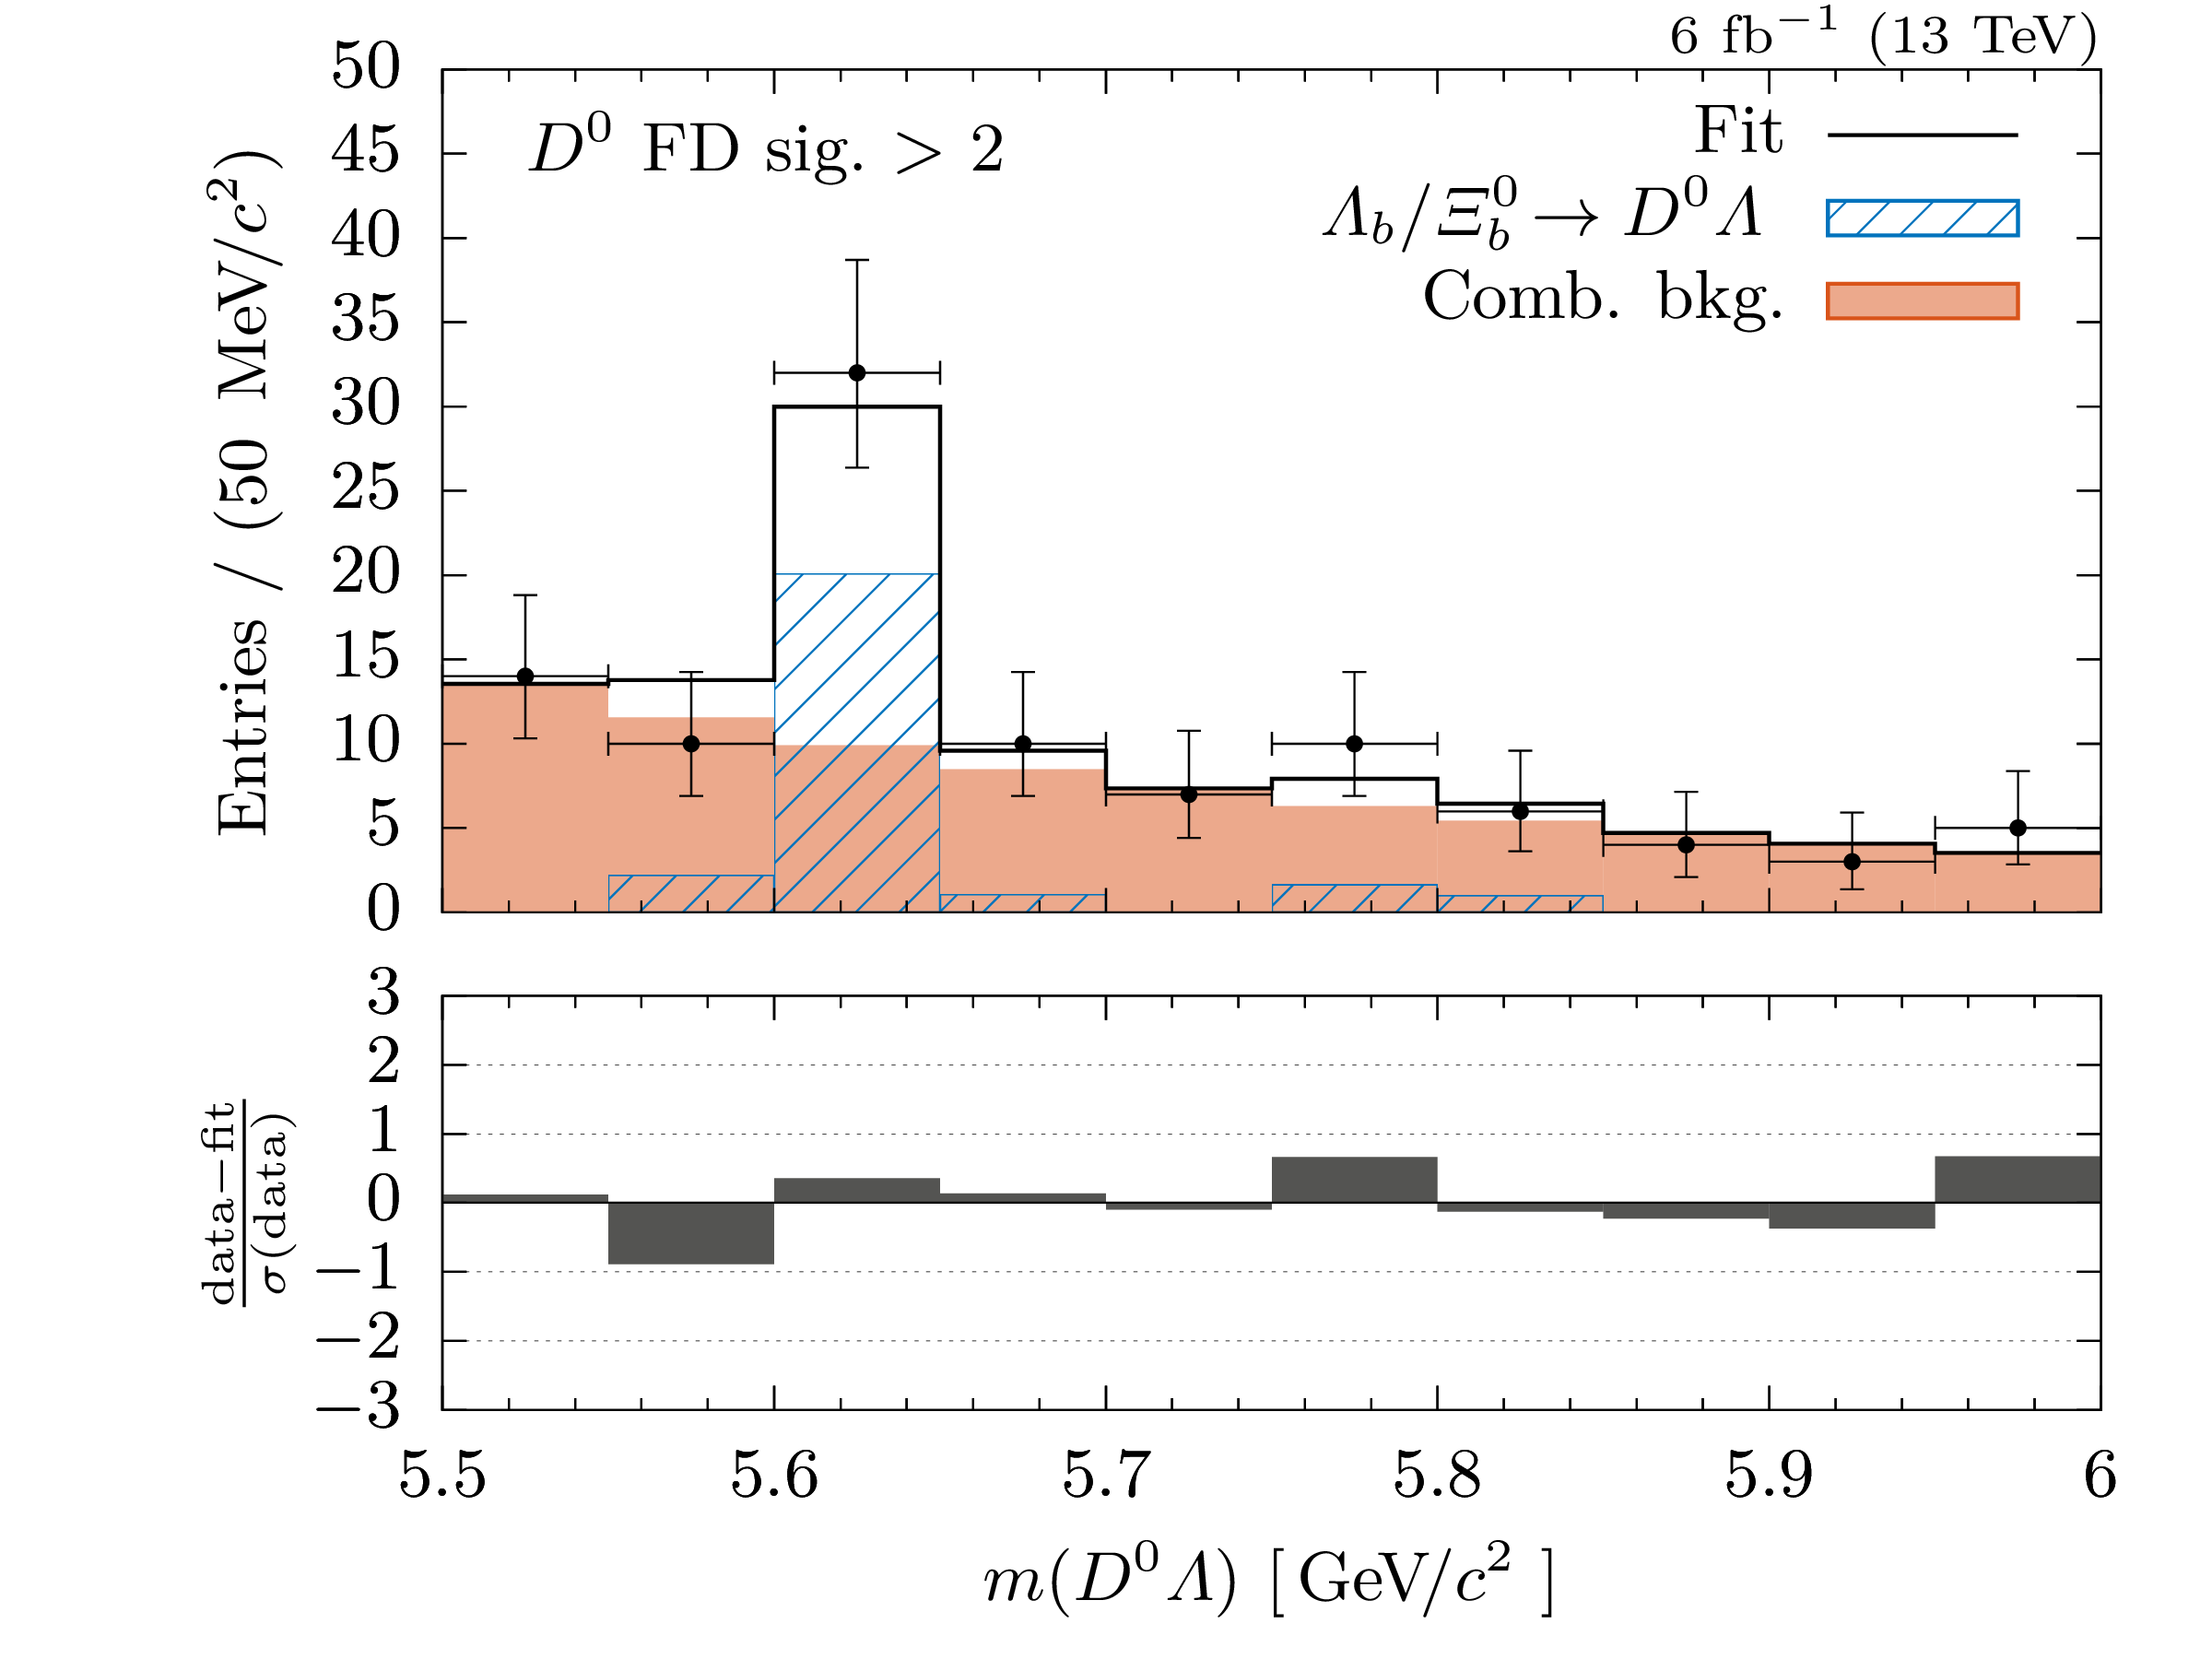
\includegraphics[scale=1.]{fit/hLbM_data_dsig2-fit.png}
    \caption{Fit to combined invariant mass of \Dz and \Lz candidates of both track types from recorded data, when the flight distance significance of \Dz candidates is required to be larger than 2.}
    \label{fig:fit_hLbM_dsig2}
\end{figure}

\begin{figure}[htbp]
    \centering
    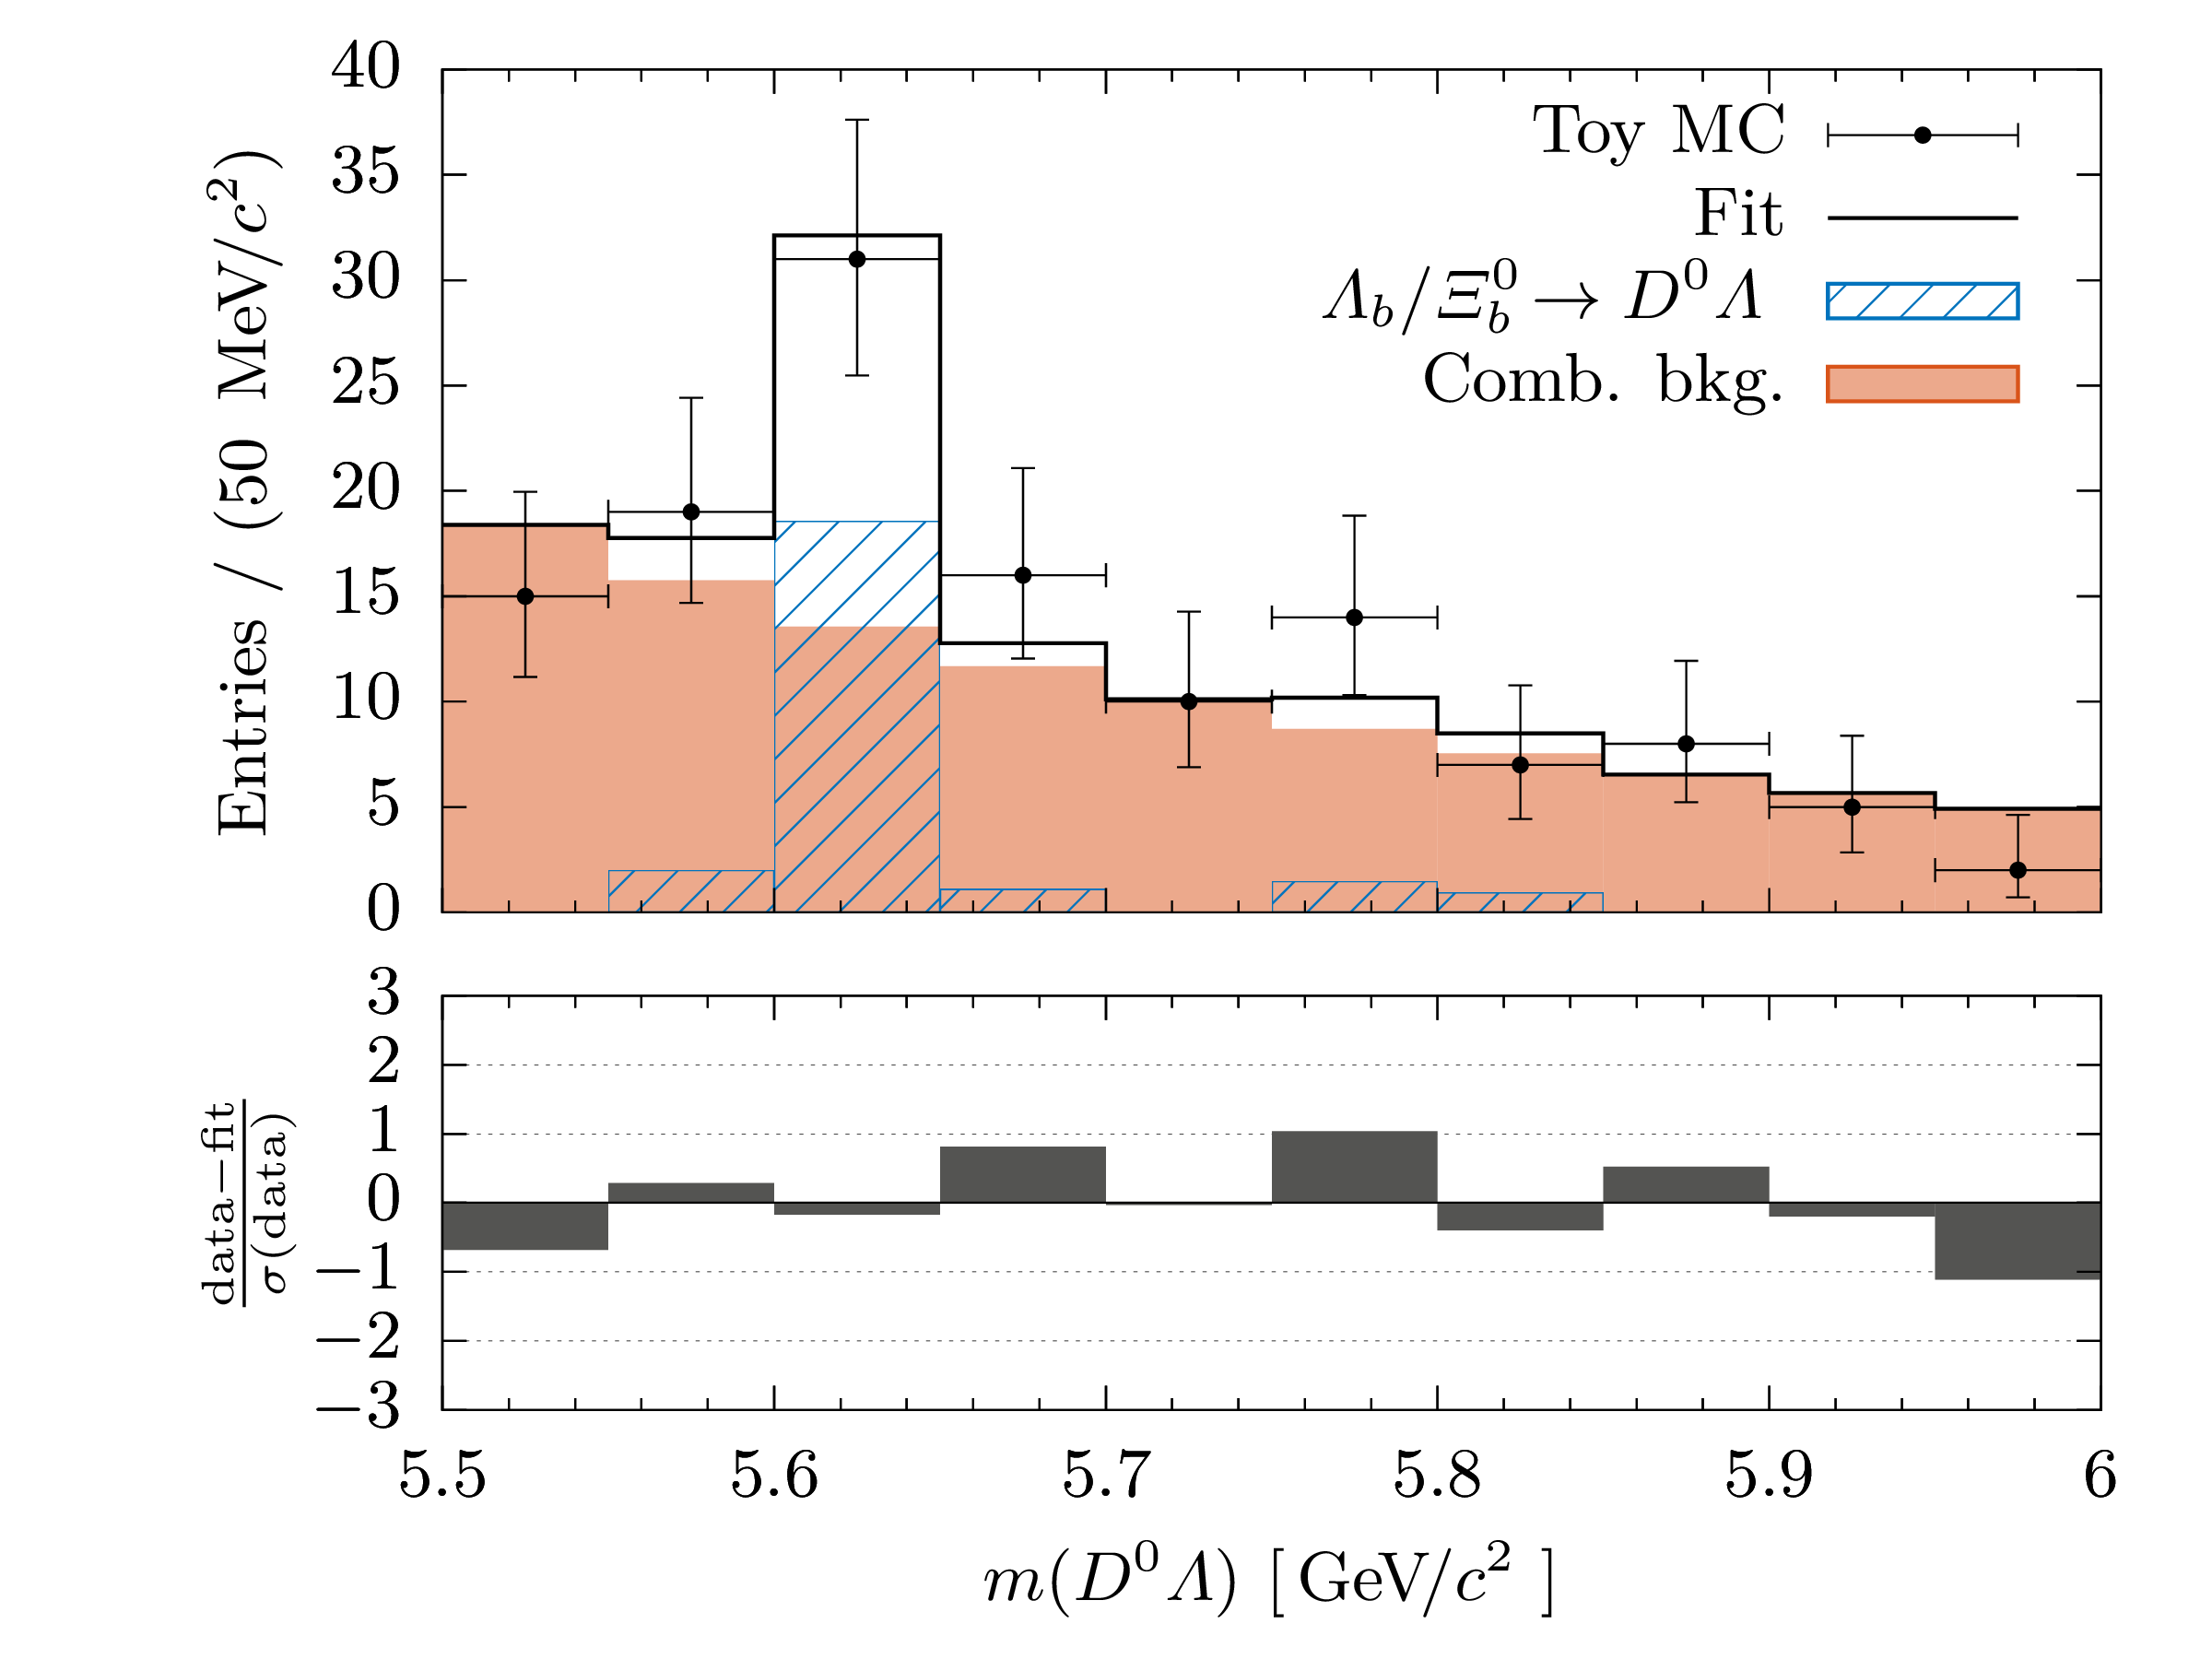
\includegraphics[scale=1.]{fit/hLbM_toy_full_fit3.png}
    \caption{Example of a distribution that was generated as part of the pseudo-experiment to test for a bias and the validity of the error estimation of the fit. For the generation and fitting both signals modes were kept enabled.}
    \label{fig:fit_hLbM_toy_full_fit3}
\end{figure}

\begin{figure}[htbp]
    \centering
    \begin{subfigure}[b]{\textwidth}
        \centering
        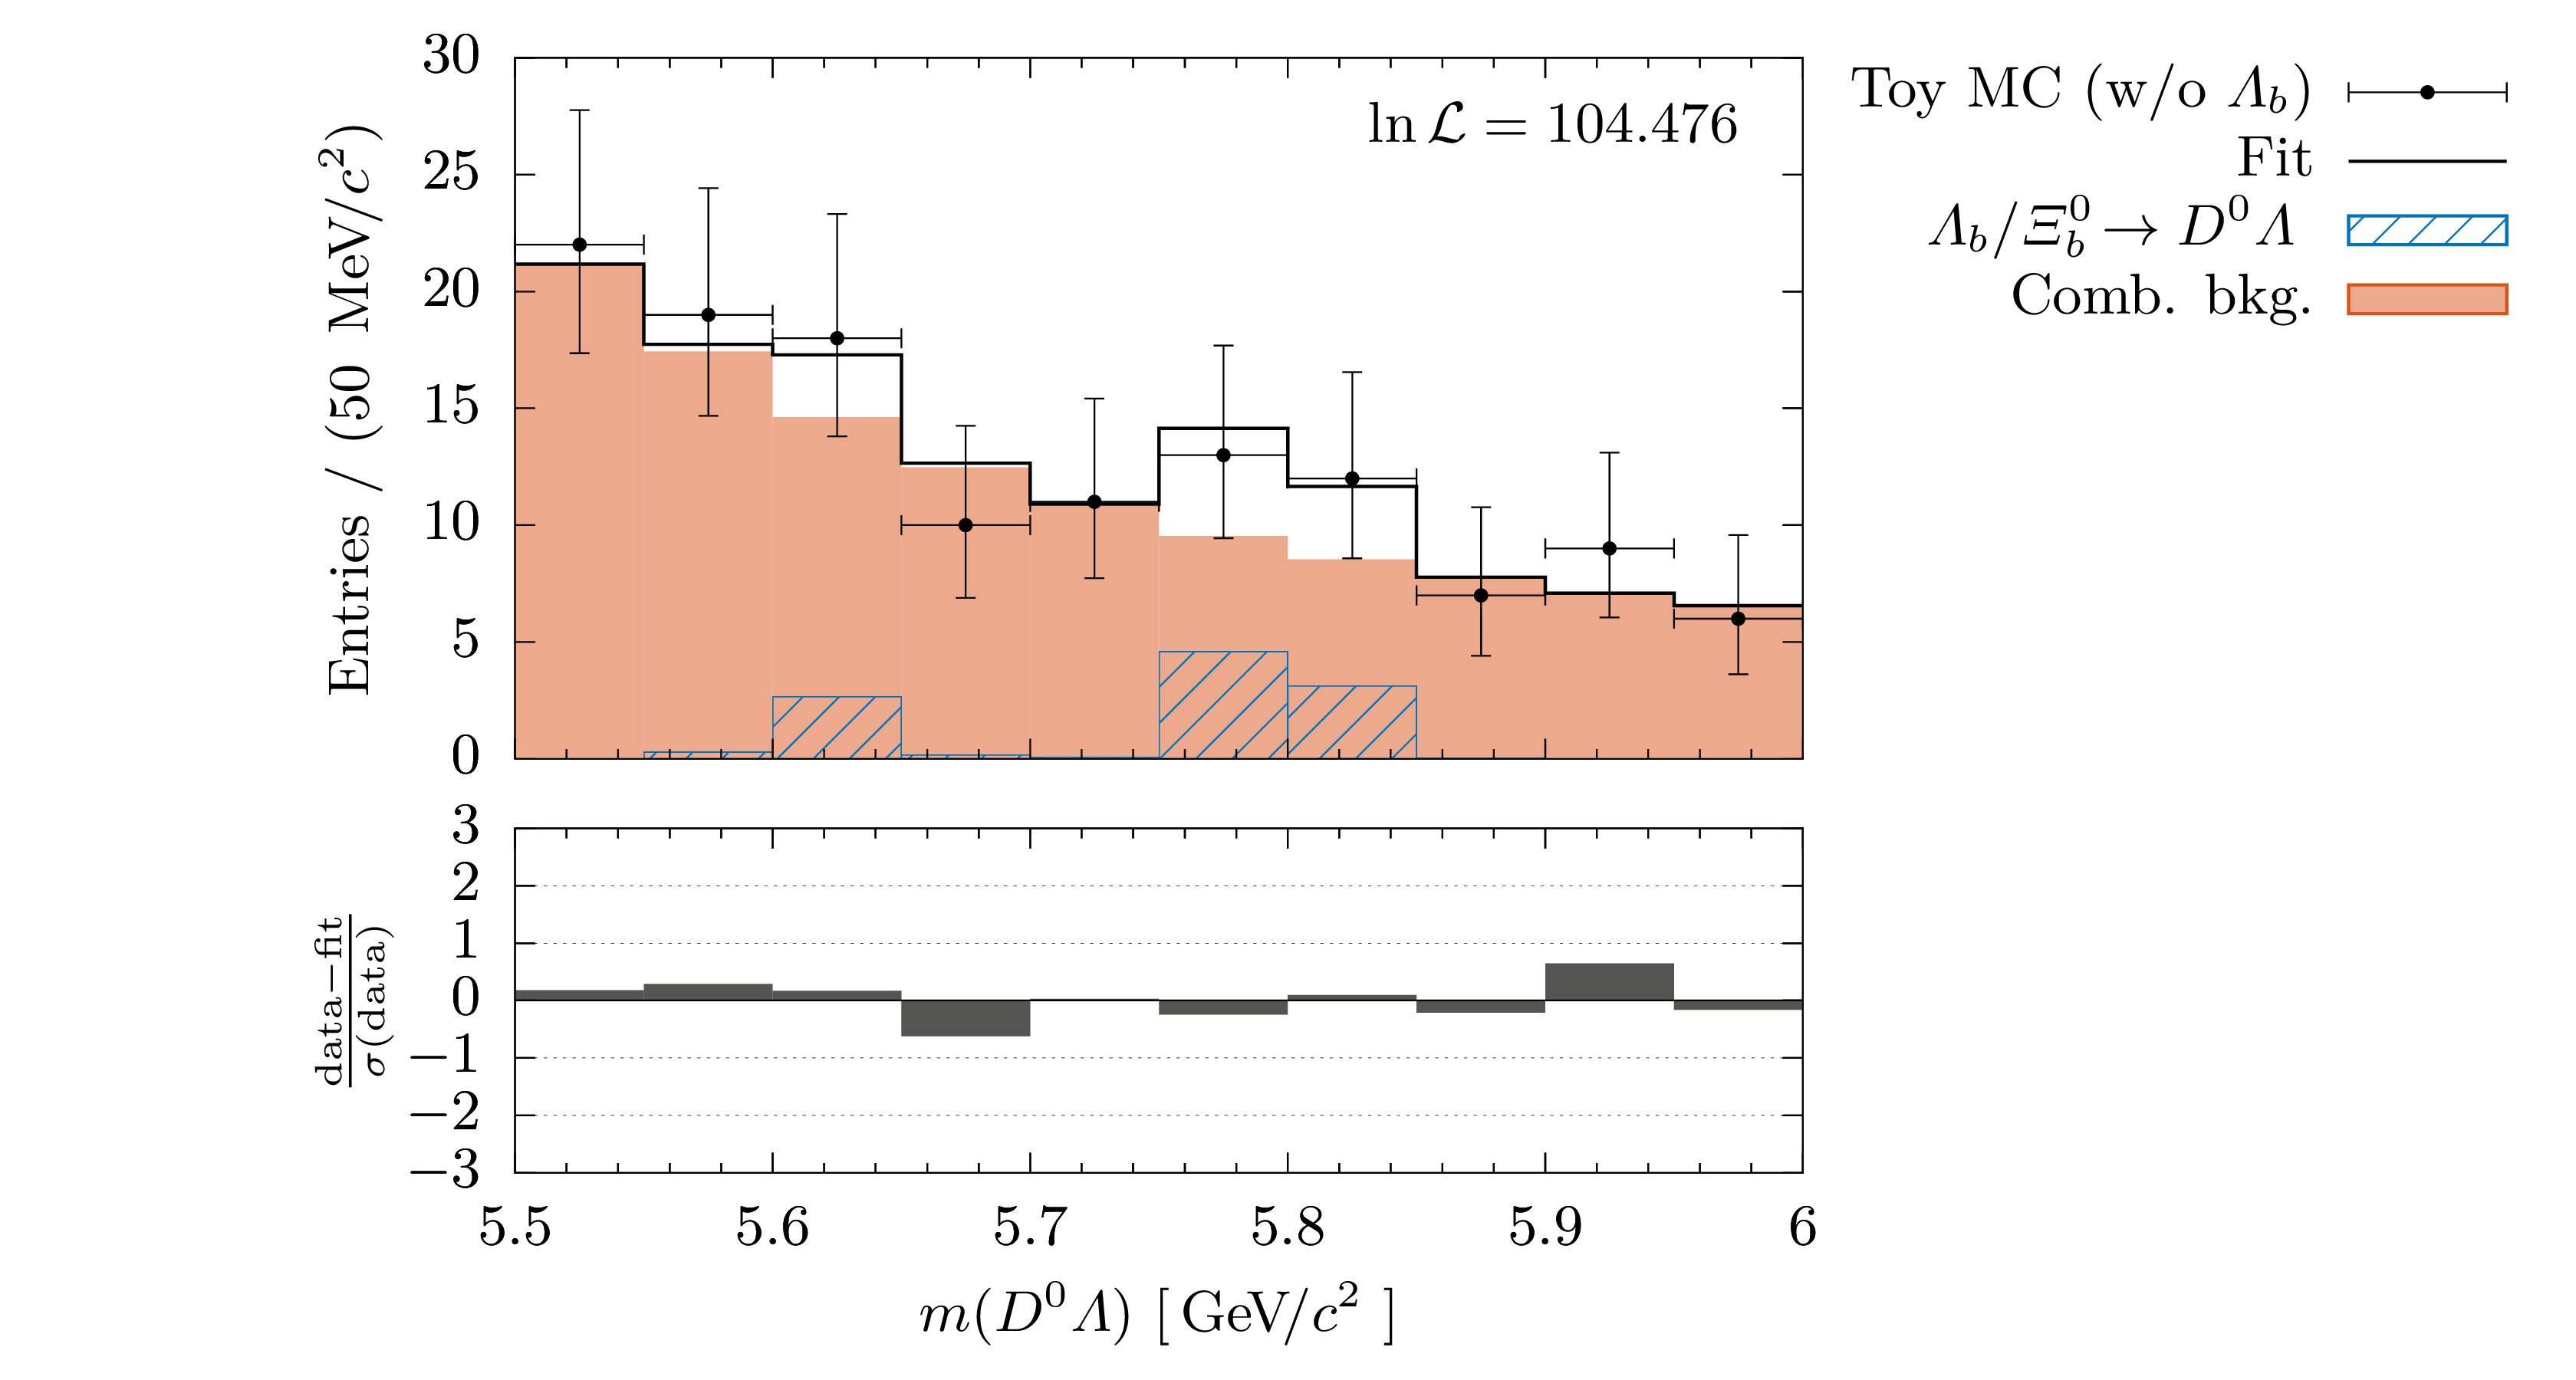
\includegraphics[scale=1.]{fit/hLbM_toy_noLb_fit1.png}
    \end{subfigure}
    \par\bigskip 
    \begin{subfigure}[b]{\textwidth}
        \centering
        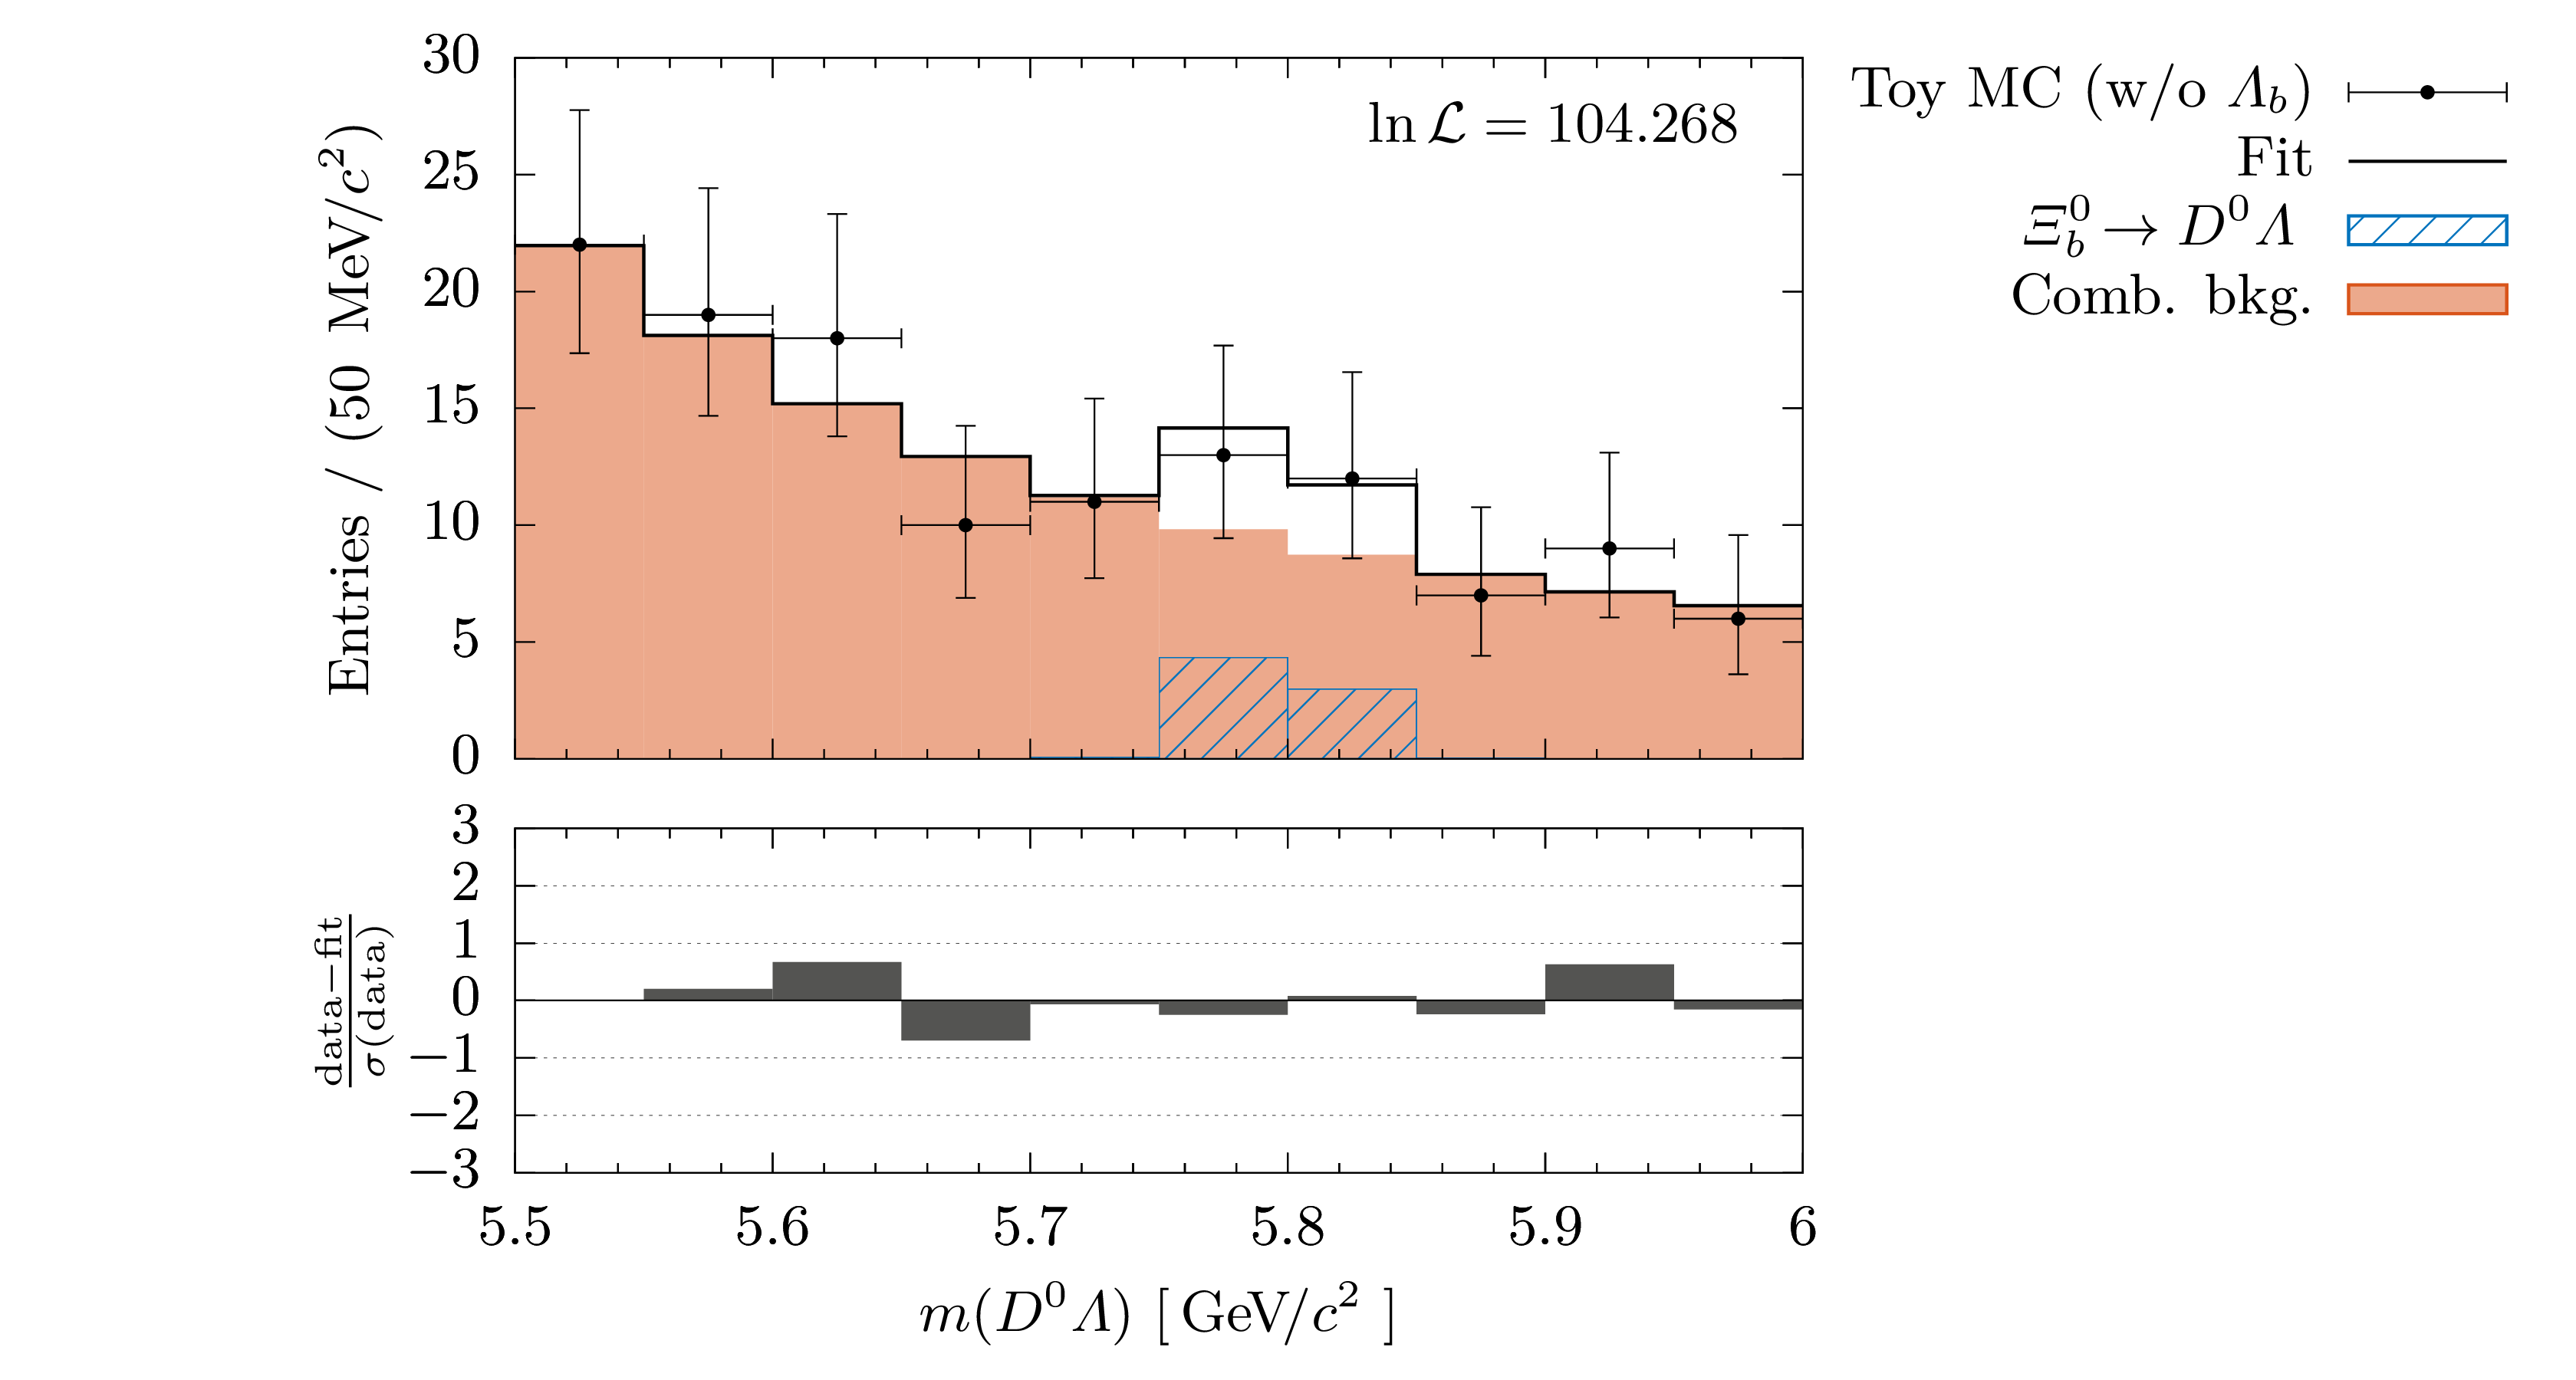
\includegraphics[scale=1.]{fit/hLbM_toy_noLb_fit2.png}
    \end{subfigure}
    \caption{Example of a distribution (data points) that was generated as part of the pseudo-experiment to test the validity of the signal yield significance of the \decay{\Lb}{\Dz\Lz} mode. During generation this mode was kept disabled (null hypothesis). The distribution is fitted twice, first with the \Lb signal component enabled (top) and once with disabled \Lb signal component (bottom). The difference in the log-likelihood values is then used to benchmark the null-hypothesis.}
    \label{fig:fit_hLbM_toy_noLb}
\end{figure}

